% !TEX root = ../../book.tex
\chapter{Univariate Time Series Models \label{ch:ch_uvts}}

With the advent of electronic trading a vast amount of data on orders is now recorded and is available to traders to make real-time decisions. The Trades and Quotes (TAQ) data on time-stamped sequence of trades with the updates on the price and depth of the best bid and ask quotes was used by researchers and traders initially. This was later expanded to the so-called Level~II data, with time-stamped sequence of trades and quotes for the top 5 levels of the order book. Both TAQ and Level~II data still do not provide the complete story of the buy and sell sides. With Level III data now available, we can obtain time-stamped sequence of all events that occur, with the exception of the information on hidden orders. Thus the data related to all trading activities is quite voluminous and is irregularly spaced. We take a broad view that for making strategic decisions to enter and exit the market, the trader needs to take an aggregate view of the trading activities, but that for the optimal execution of the strategies the trader needs to understand the market micro-structure that relates to the actual process of trading. With the increased speed of decisions that are made nowadays the difference between the two steps, strategic and execution decisions may be blurred, but the aggregation process may help to look beyond trading frictions. In Section~\ref{sec:tradesandquotes}, we discuss the Trades and Quotes data and the aggregation issues. In Section~\ref{sec:trad_dec_stfd}, we define that the trading algorithms depend on prediction of short-term price movement.


The price movement whether it is due to pure market friction or due to information related to a stock is captured through a drift term in the random walk model that needs to be carefully monitored. Because time series models for discrete time units are still widely used by the traders in the form of aggregated price-bars, we focus on these methods in Sections~\ref{sec:modelingthemean} to Section~\ref{sec:sty_mod_var}. We broadly classify these methods into modeling the mean (return) and into modeling the variance (volatility). As these techniques are well-documented and can be found elsewhere in the literature, we only present a brief but relevant overview. The established facts about the stock returns and variances are reviewed along with the methodology as these will provide expected benchmarks; successful algorithms as one would notice, generally exploit the deviations from these benchmarks.



% Trades and Quotes Data and their Aggregation
\section{Trades and Quotes Data and their Aggregation: From Point Processes to Discrete Time Series \label{sec:tradesandquotes}}

In its simplest form, the trading activities of equity through an exchange that opens at 9:30~a.m. and closes at 4~p.m. can be described by a sequence of time stamps (``ticks'') $t_0 < t_1 < \cdots < t_n$ and the ``marks'' $y_i$ at time $t_i$, in which $t_0$ denotes 9:30~a.m. and after and $t_n$ denotes the time of the last trade that occurs before or at 4~p.m. The marks $y_i$ can be price, volume of an order placed on either the buy or sell side of the trade and in general can represent the characteristics of the order book at the time of $i$th activity (see Figure~\ref{fig:tradeactline}). The events with the marks associated with the ticks can be described mathematically as a marked point process. But our goal here is to first show how these data can be aggregated over regularly spaced time intervals and how methods for linear homogeneous time series can be used to analyze the aggregated data. Some tools that are relevant for the analysis of point processes will be presented in Chapter~\ref{ch:ch_advanced}.	
	\begin{figure}[!ht]
	\centering
	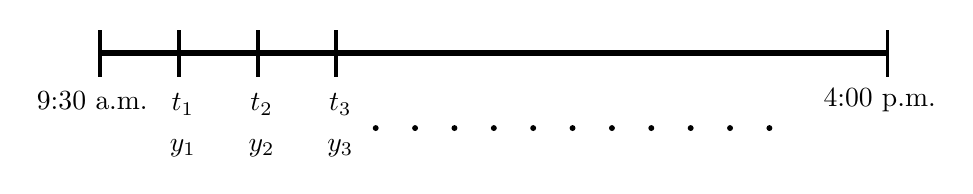
\begin{tikzpicture}
	\draw[line width=0.08cm] (-5,0) -- (5,0);
	
	\draw[line width= 0.05cm] (-5,-0.3) -- (-5,0.3);
	
	\draw[line width = 0.05cm] (-4,-0.3) -- (-4,0.3);
	\draw[line width = 0.05cm] (-3,-0.3) -- (-3,0.3);
	\draw[line width = 0.05cm] (-2,-0.3) -- (-2,0.3);
	
	\draw[line width=0.05cm] (5,-0.3) -- (5,0.3);
	
	\node at (-5.1,-0.6) {9:30 a.m.};
	\node at (4.9,-0.6) {4:00 p.m.};
	
	\node at (-3.95,-0.65) {$t_1$};
	\node at (-2.95,-0.65) {$t_2$};
	\node at (-1.95,-0.65) {$t_3$};
	
	\node at (-3.95,-1.2) {$y_1$};
	\node at (-2.95,-1.2) {$y_2$};
	\node at (-1.95,-1.2) {$y_3$};
	
	\foreach \xcoord in {-1.5,-1.0,...,3.8} 
	{
	\draw[fill] (\xcoord,-0.95) circle (0.03cm);
	}
	\end{tikzpicture}
	\caption{Trading Activities. \label{fig:tradeactline}}
	\end{figure}


The typical Level~III data for CISCO on a single day in 2011 is given below in Table~\ref{tab:CISCO}. This outlay in Table~\ref{tab:CISCO} points to various issues that need to be addressed in processing this type of data. The order numbers are only unique during the lifetime of the order but can be reassigned at a later time. Several activities such as submissions, cancellation or modification of an order, all can take place at the same time stamp. Hidden orders are revealed only when they are executed and as such do not have visible order numbers. Full cancellation quantity and price information should be traced back to the submission time. To summarize, at any given point in time using the data described in Table~\ref{tab:CISCO}, the full limit order book that essentially records where each order is in the queue, can be constructed and thus providing the activity time and the associated marks. These and other characteristics of the limit order book (superbook---if we collate this information from all exchanges) will be taken up in a later chapter, but the focus here is on constructing discrete time series data from this point process data. 
	\begin{table}[!ht]
   	\centering
   	\caption{CISCO--Trade Data \label{tab:CISCO}}
   	\begin{tabular}{cccccc} 
	Timestamp & Order Number & Event & Quantity & Price & Exchange \\ \hline
	$\vdots$ & $\vdots$ & $\vdots$ & $\vdots$ & $\vdots$ & $\vdots$ \\
	34561915 & 4254917 & D & 0 & 0 & J \\
	34561915 & 4253917 & B & 200 & 20.55 & J \\
	$\vdots$ & $\vdots$ & $\vdots$ & $\vdots$ & $\vdots$ & $\vdots$ \\
	34561923 & 13056048 & S & 200 & 20.58 & Z \\
	$\vdots$ & $\vdots$ & $\vdots$ & $\vdots$ & $\vdots$ & $\vdots$ \\
	34573369 & 13255731 & C & 98 & 0 & Q \\
	$\vdots$ & $\vdots$ & $\vdots$ & $\vdots$ & $\vdots$ & $\vdots$ \\
	34577331 & 6225085 & E & 300 & 0 & K \\
	$\vdots$ & $\vdots$ & $\vdots$ & $\vdots$ & $\vdots$ & $\vdots$ \\
	34577338 & 6225085 & F & 0 & 0 & K \\
	$\vdots$ & $\vdots$ & $\vdots$ & $\vdots$ & $\vdots$ & $\vdots$ \\
	34573379 & 2030057 & S & 100 & 20.77 & K \\
	$\vdots$ & $\vdots$ & $\vdots$ & $\vdots$ & $\vdots$ & $\vdots$ \\
	34573382 & NA & T & 1700 & 20.37 & P \\
	$\vdots$ & $\vdots$ & $\vdots$ & $\vdots$ & $\vdots$ & $\vdots$ 
   	\end{tabular}
	\begin{minipage}[t]{1\textwidth}
	\small{*Time-stamp is the time since midnight; Event: B: submission of LO on Buy side; S: submission of LO on sell side; T: full execution of a LO; F: full execution of a LO; E: partial execution of a LO; D: full cancellation of a LO; C: partial cancellation of a LO; Exchange: Q-NASDAQ; J-EDGE-A; Z-BATS-Z; K-EDGE-K; P-ARCA; etc}
	\end{minipage}
	\end{table}


To illustrate the aggregation methods, we will initially focus on price of the stock, $P_t$, and the associated volume $V_{t}$. Two types of aggregation methods are proposed in the literature. One when the time span $T$ for the Exchange hours (9:30~a.m.--4:00~p.m.) is divided into `$K$' intervals so that the regularly spaced intervals are of size $\Delta t = T/K$. The other method will do aggregation when there is a change in a marker, such as price. Here we focus on the first method. Various summary measures within each period $((i - 1)\Delta t, i\Delta t)$ where $i = 0,1,\ldots,K$ can be computed;
        \begin{itemize}
        \item number of transactions: `$n_i$'
        \item Average price: $\overline{P}_i = \sum P_{t_j}/n_i$
        \item Volume Weighted Average Price: $\overline{P}_{wi} = \sum V_{t_j} P_{t_j}/ \sum V_{t_j}$
        \item Average duration between transactions: $\overline{d}_i = \sum_{j\in ((i-1)\Delta t,i\Delta t) }(t_j - t_{j-1})/n_i$
        \item Mid-Price: $(\text{Best bid}_i+\text{Best ask}_i)/ 2$
        \end{itemize}


The typical daily data (also called price bars) that is available from popular sources such as Yahoo finance provide information on opening, closing, high and low prices along with the volume. This type of aggregation can also be done for shorter duration, such as five minutes and this largely results in smoothed data that can cancel out short term market frictions and yet capture the price variations that may be due to information. 


It is possible that for infrequently traded stocks, some time intervals may not contain any trading activity. For heavily traded stocks, the duration can be very small and thus may not provide any consequential information. We will discuss this further in Chapter~\ref{ch:ch_advanced}. To begin with, we present the analysis for data aggregated over fixed time intervals. Depending on the size of the interval, the data can be called low frequency or high frequency but the time series methods that are discussed in this chapter apply to \emph{all} aggregated data.



% Trading Decisions as Short-Term Forecast Decisions
\section{Trading Decisions as Short-Term Forecast Decisions \label{sec:trad_dec_stfd}} 


Most trading decisions generally involve the following considerations
        \begin{itemize}
        \item How much to trade?
        \item When to trade, i.e. when to enter and when to exit?
        \item How to trade? How fast? What is the objective? What are the benchmarks?
        \end{itemize}
Answers to these questions involve in some way predicting the market movement and in particular the future (short-term and long-term) price of assets. In the short term it is possible that prices have a tendency to `trend' or exhibit `momentum' but in the long run, prices have a tendency to `mean-revert' as the information about the asset gets incorporated into the price. 


Let $p_{it}= \ln P_{it}$ denote the price of the $i$th asset at time $t$ and let $p_t = (p_{1t}, p_{2t}, \ldots, p_{nt})$ denote the price vector for `$n$' assets. Let $y_{it}$ denote a vector of characteristics, e.g. volume of transactions, price volatility, number of transactions and the intensity of trading as captured by the average duration between transactions, etc of the $i$th asset at time $t$. These quantities are aggregated from high-frequency data of type given in Table~\ref{tab:CISCO} and illustrated in Figure~\ref{fig:tradeactline} to be used as the characteristics associated with the price changes. In addition, we can also consider $r$ factors $f_t = (f_{1t}, f_{2t}, \ldots, f_{rt})$ that may include market and industry factors as well as asset characteristics such as market capitalization, book-to-market ratio etc. The trading rules can be broadly grouped as follows:
        \begin{itemize}
        \item[A.] Statistical Arbitrage Rules: $E(p_{i,t+1}\,|\,p_{i,t},p_{i,t-1},\ldots,y_{i,t},y_{i,t-1},\ldots)$
        \begin{itemize}
        \item[$\bullet$] Predicting the price of $i$th stock at t+1 based on the past trading information; this is sometimes labelled as time series momentum.
        \end{itemize}
        \item[B.] Momentum: $E(p_{t+1}\,|\,p_{t},p_{t-1},\ldots,y_{t},y_{t-1},\ldots)$
        \begin{itemize}
        \item[$\bullet$] Predicting the cross-sectional momentum of a subset of stocks based on their past trading characteristics. This is not only useful for portfolio formation and rebalancing, also for pairs trading which is based on tracking two stocks simultaneously so that their price divergence can be exploited. 
        \end{itemize}
        \item[C.] Fair Value: $E(p_{t+1}\,|\,p_{t},p_{t-1},\ldots,y_{t},y_{t-1},\ldots,f_t,f_{t-1},\ldots)$
        \begin{itemize}
        \item[$\bullet$] Predicting the price using all relevant quantities. The factors normally include market and Farma-French factors. Many of these factors are at a more macro level than the time scale considered for the price prediction, but nevertheless could be useful, as explained in Chapter~\ref{ch:ch_mvts}.
        \end{itemize}
        \end{itemize}
\noindent Thus the price (or alternatively, return) and volatility (or squared return) prediction can be formulated as a time series prediction problem and the common tools such as autocorrelations and partial autocorrelations can be used to build autoregressive and ARCH models that are shown to have some predictive power. 


Predicting stock market behavior has been studied extensively starting in the early 20th century. Cowles (1933, 1944)~\cite{cow1,cow2} evaluated the performance of the stock market forecasters. Analyzing the performance of several financial services that made some 7500 recommendations on common stocks over a period, January 1, 1925 to July 1, 1952, it was pointed out the record was worse than the performance of average common stock by 1.43\% annually. Thus `buy-and-hold' strategy out-performed the stock picking strategies of those days. In fact, a much harsher assessment is made: ``A review of the various statistical tests, applied to the records for this period, of these 24 forecasters, indicates that the most successful records are little, if any, better than what might be expected to result from pure chance. There is some evidence, on the other hand, to indicate that the least successful records are worse than what could reasonably be attributed to chance.'' Many of these comments are still valid and have stood the test of the time. Yet, we will demonstrate in this book that there are opportunities for statistical arbitrage. The key is to have access to relevant information and use the appropriate techniques to exploit the information in a timely manner. 



% Time Series Models for Aggregated Data
\section{Time Series Models for Aggregated Data: Modeling the Mean \label{sec:modelingthemean}}

In this section, we present a broad overview of the time series models for data aggregated over discrete time intervals. This data as mentioned in Section~\ref{sec:tradesandquotes} is called price bars and the methodologies discussed in Section~\ref{sec:modelingthemean} here apply to any aggregated data for fixed time unit of aggregation that is of equal length. As a close substitute for the high frequency data, data aggregated over short intervals such as two or five minutes can be used.



% Stochastic Processes
\subsection{Stochastic Processes: Some Properties}

Formally, a discrete time series or stochastic process $Y_1, Y_2, \ldots, Y_T$ is a sequence of random variables (r.v.'s) possessing a joint probability distribution. A particular sequence of observations of the stochastic process $\{ Y_t, t=1, \ldots,  \, T\}$ is known as a realization of the process. For such a collection of r.v.'s, the joint distribution function is defined by
	\begin{equation} \label{eqn:feqnfirst}
	F_{12 \ldots T}\left(y_1, y_2, \ldots,  \, y_T\right)= \text{Pr}[Y_1 \leq y_1, Y_2 \leq y_2, \ldots,  	\, Y_T \leq y_T]
	\end{equation}
In general, determining the properties and identifying the probability structure which generated the observed time series are of interest. We do not attempt to study the joint distribution of $Y_1, Y_2, \ldots, \, Y_T$ directly, as it is too complicated for large $T$, but we study the probabilistic mechanism which generates the process sequentially through time, and from this we derive the conditional distribution of future observations for purposes of prediction.


Because the means, variances, and covariances are useful summary descriptions of the joint probability distribution of the stochastic process $\{ Y_t, t=1, \ldots,  \, T\}$, we will consider these quantities that are functions of $t$:
	\begin{equation} \label{eqn:texteqn}
	\begin{split}
	\text{mean, } \mu(t)&= E(Y_t) \\
	\text{variance, } \sigma^2(t)&= \var(Y_t)= E[(Y_t - \mu(t))^2] \\
	\text{autocovariance, } \gamma(t,s)&= \cov(Y_t,Y_s)= E[(Y_t-\mu(t))(Y_s - \mu(s))] \\
	\text{autocorrelation, } \rho(t,s)&= \corr(Y_t,Y_s)= \dfrac{\gamma(t,s)}{\sigma(t)\sigma(s)}
	\end{split}
	\end{equation}
It is not possible to estimate the unknown parameters (means, variances, and covariances) from a single realization of $T$ observations. In addition, such generality in the specification of the mean and covariance structure is not of much use for the prediction of future observations of the process. Hence we must impose some additional structure on the joint distribution of the process in order to substantially reduce the number of unknown parameters. The concept of stationarity of a process serves as a realistic assumption for many types of time series. Stationarity is motivated by the fact that for many time series in practice, segments of the series at different points in time behave similarly. \\


\noindent \textbf{Stationarity} \\


A time series $\{Y_t \}$ is said to be stationary if for every integer $m$ the set of variables $Y_{t_1}, Y_{t_2}, \ldots, \, Y_{t_m}$ depend only on the distance between the times $t_1, t_2, \ldots, t_m$, rather than on their actual values.  So a stationary process $\{Y_t \}$ tends to behave in a homogeneous manner as it moves through time. The means and variances of the $Y_t$ are the same for all $t$, that is, $E(Y_t) = \mu$ and  $\var(Y_t)= \sigma^2$ are constant, for all $t$. So we may express the autocovariance function as 
	\begin{equation} \label{eqn:2gammas}
	\gamma(s)= \cov(Y_t,Y_{t - s})= E[(Y_t - \mu)(Y_{t - s} - \mu)], \text{ for all } s= 0, \pm 1, \ldots
	\end{equation}
Note that by this notation, $\gamma(0) = E[(Y_t - \mu)^2] = \var(Y_t)$. Also, the \emph{autocorrelation function} of the stationary process may be expressed
        	\begin{equation} \label{eqn:2rhos}
	\rho(s)= \corr(Y_t,Y_{t - s})= \dfrac{\cov(Y_t,Y_{t - s})}{\big( \var(Y_t) \var(Y_{t-s}) \big)^{1/2}} = \dfrac{\gamma(s)}{\gamma(0)},  \quad  s= 0, \pm 1, \ldots
	\end{equation}
$\rho(s)$ will be referred to as the autocorrelation of the process at lag $s$. The autocorrelation function (ACF), $\rho(s)$ of a stationary process $\{Y_t\}$ is a very important tool in describing the characteristics of the process, because it is a convenient summary of the correlation structure of the process over time lags.  \\


\noindent \textbf{Examples of Stationary Stochastic Processes} \\


Now we present some select models as examples, because they are the most relevant to financial applications. The properties of these models would become relevant as we look at data. 


\begin{ex}[White Noise] \label{ex:whitenoise} Let $\epsilon_0, \epsilon_1, \epsilon_2, \ldots$ be a sequence of independent random variables defined on the discrete time points $0,1, 2, \ldots$, with mean $E(\epsilon_{t})= 0$ and variance $E(\epsilon_{t}^2)= \sigma^2$, for all $t$. Set $Y_t = \mu + \epsilon_t, \, t= 0, 1, 2, \ldots$. Then $E(Y_t)= \mu$ for all $t$, and since independence implies that the random variables are uncorrelated, we have $\cov(Y_t,Y_{t-s})= \var(Y_t)= \sigma^2$ if $s=0$ and $\cov(Y_t,Y_{t-s})= 0$ if $s \neq 0$. Thus the process is stationary. Such a process is referred to as purely random process or a \emph{white noise process}, and is the foundation for the construction of many other processes of interest. \xqed
\end{ex}


\begin{ex}[Moving Average] \label{ex:movingaverage} Let $\{ \epsilon_t \}$ be independent r.v.'s as in Example~\ref{ex:whitenoise}, and define a new process $\{ Y_t \}$ by
	\[
	Y_t = \mu + \epsilon_t + \epsilon_{t-1}, \qquad t=0, 1, 2, \ldots,
	\]
where $\mu$ is a constant.  Then $E(Y_t)= \mu$, for all $t$, and
	\[
	\cov(Y_t,Y_{t-s})= \gamma(s) =
	\begin{cases}
	2 \sigma^2 & \text{if } s= 0 \\
	\sigma^2 & \text{if } s= 1 \\
	0 & \text{if } s > 1
	\end{cases}
	\]
which depends only on the time lag $s$ and not on $t$.  Hence the process $\{ Y_t \}$ is stationary with ACF $\rho(s)= \gamma(s)/\gamma(0)$ such that $\rho(0)= 1$, $\rho(1)= 1/2$ and $\rho(s)= 0$ for $|s|>1$.
 
	\begin{sidewaysfigure}[hbp]
	%\centering
                \subfloat[Figure 1a]
                        [Time series plot of $0.5 + \epsilon_t$]
                        {
                        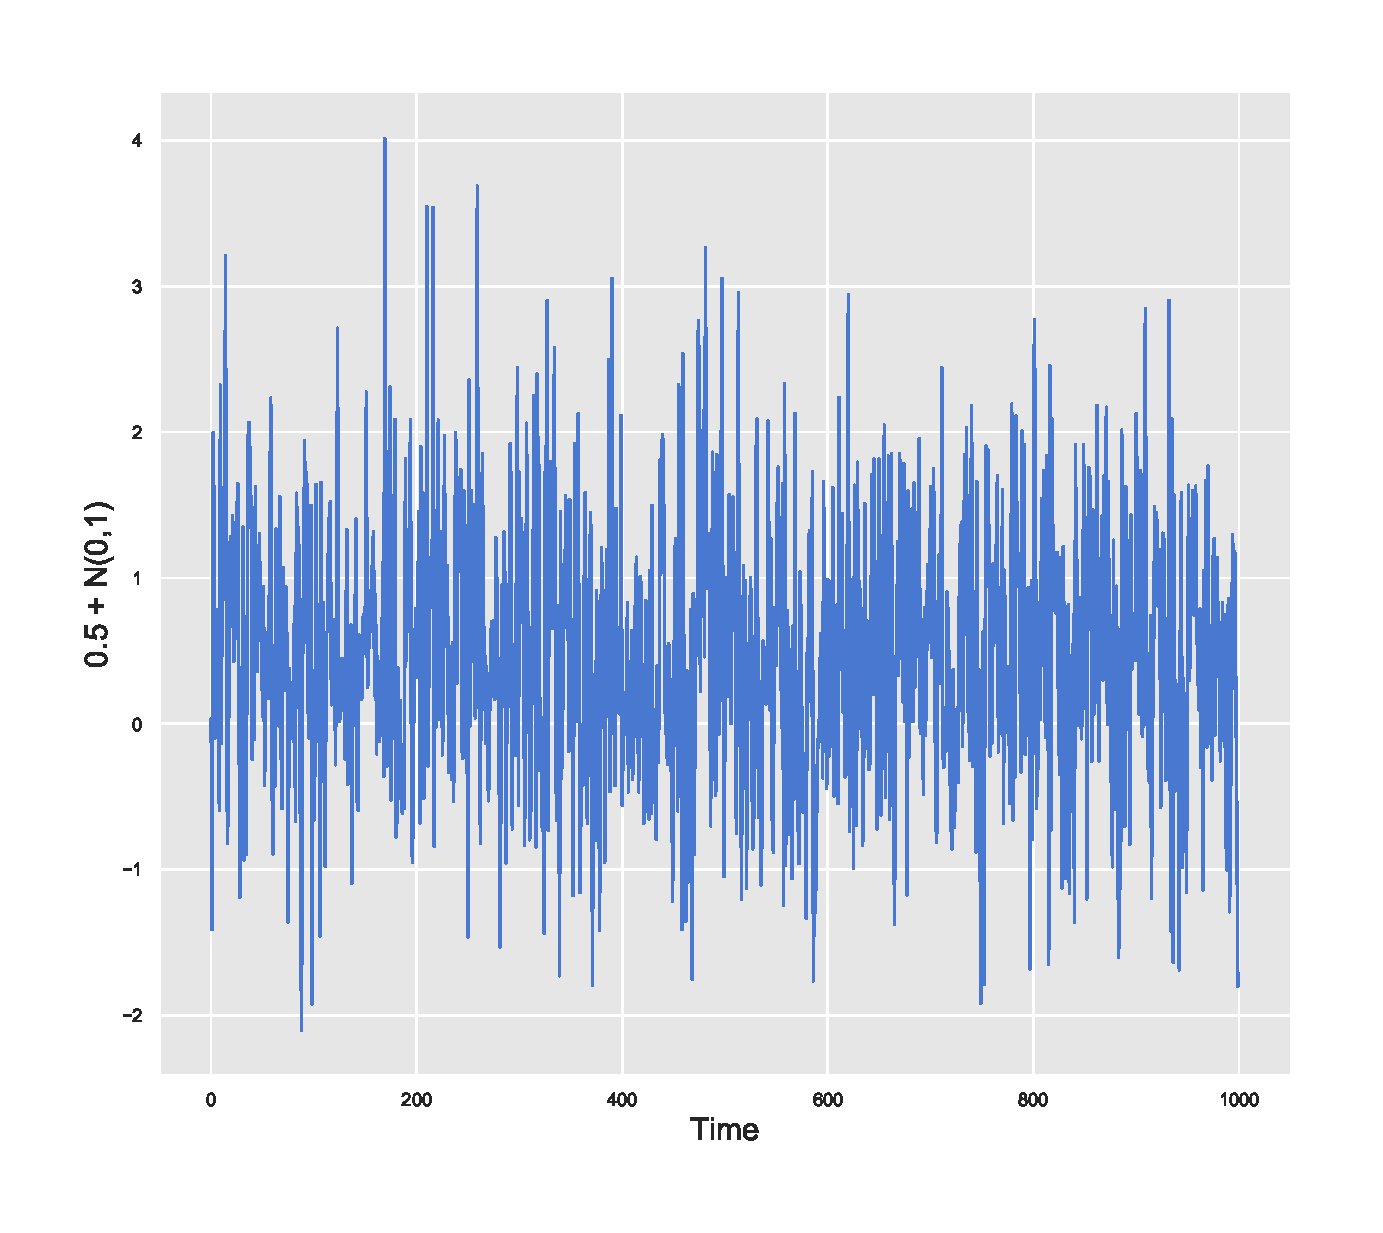
\includegraphics[scale=0.26]{chapters/chapter_uvts/figures/ch1fig1y1ts.eps}
                        }
                        \hfill
                \subfloat[Figure 1b]
                        [ACF]
                        {
                        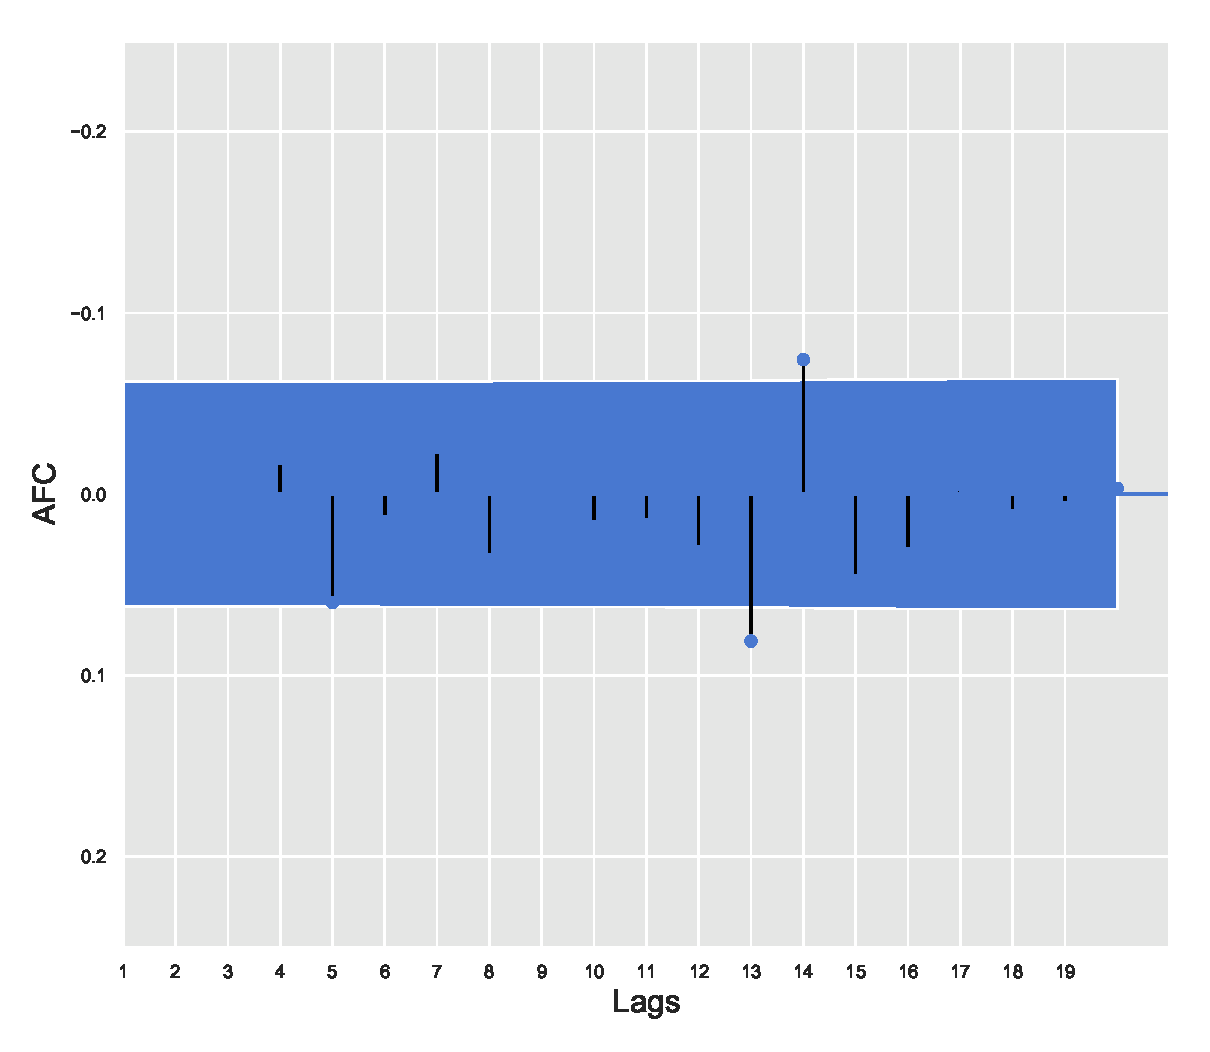
\includegraphics[scale=0.26]{chapters/chapter_uvts/figures/ch1fig1y1acf.eps}
                        }
                        \hfill
                \subfloat[Figure 1c]
                        [$Y_t$ vs. $Y_{t-1}$]
                        {
                        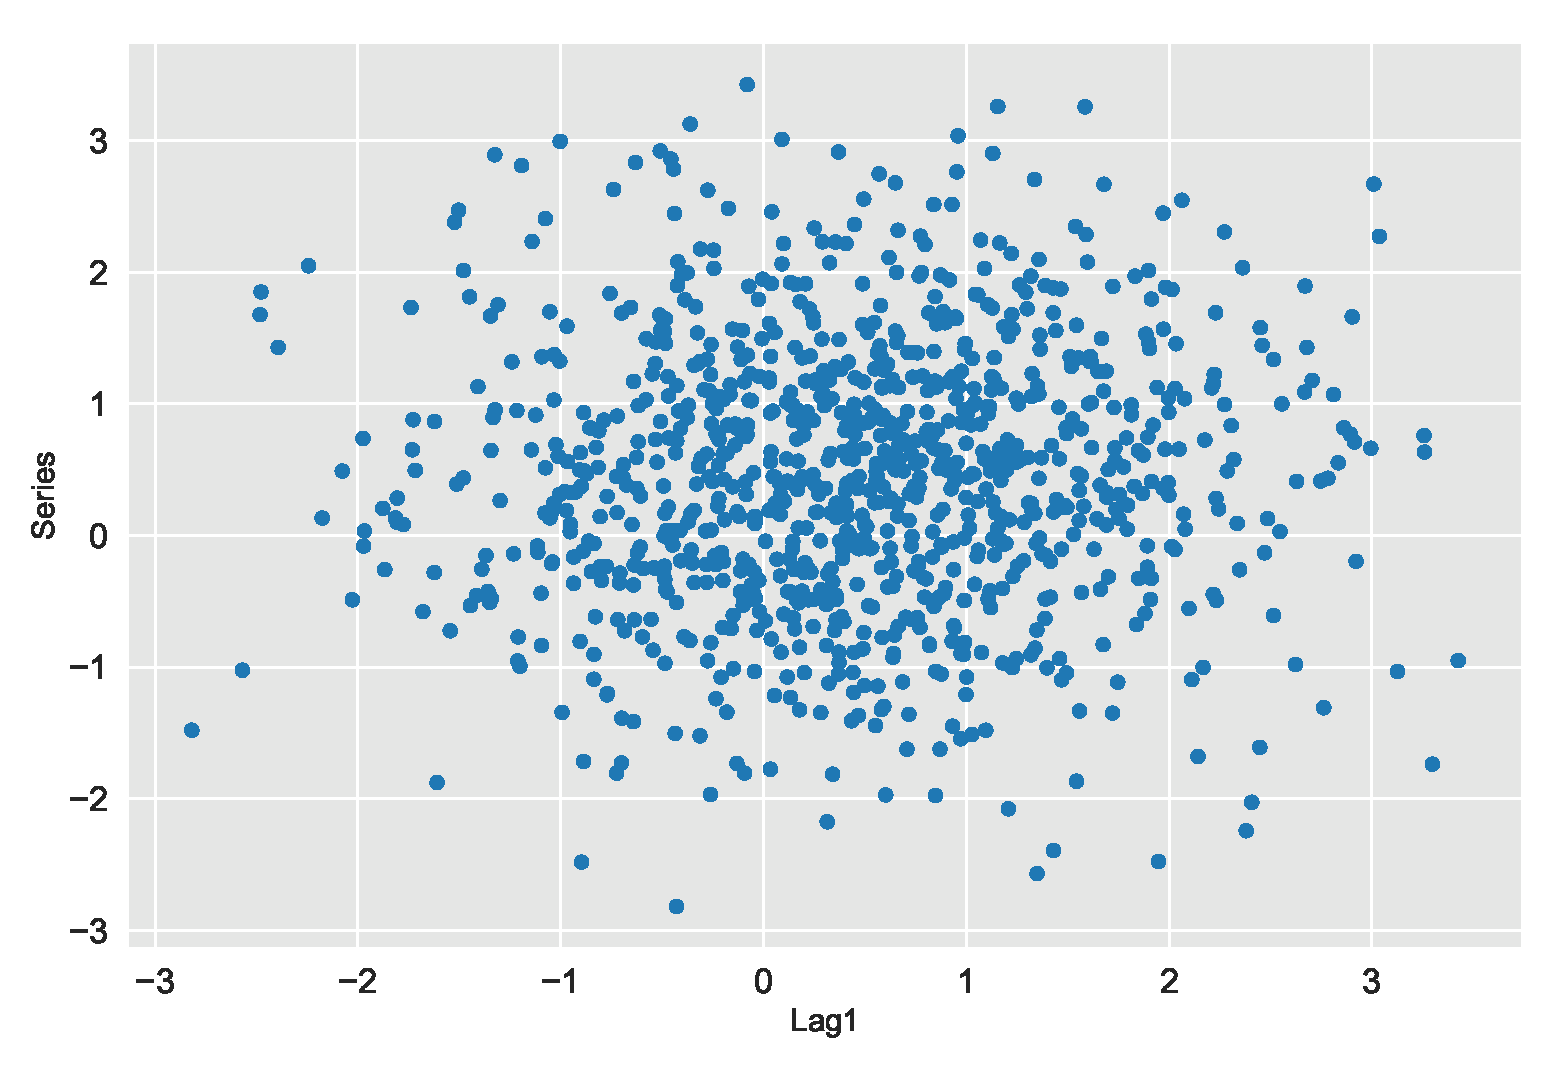
\includegraphics[scale=0.26]{chapters/chapter_uvts/figures/ch1fig1y1lagplot.eps}
                        }
                \quad
                \subfloat[Figure 1d]
                        [Time series plot of $1.0 + \epsilon_t + \epsilon_{t-1}$]
                        {
                        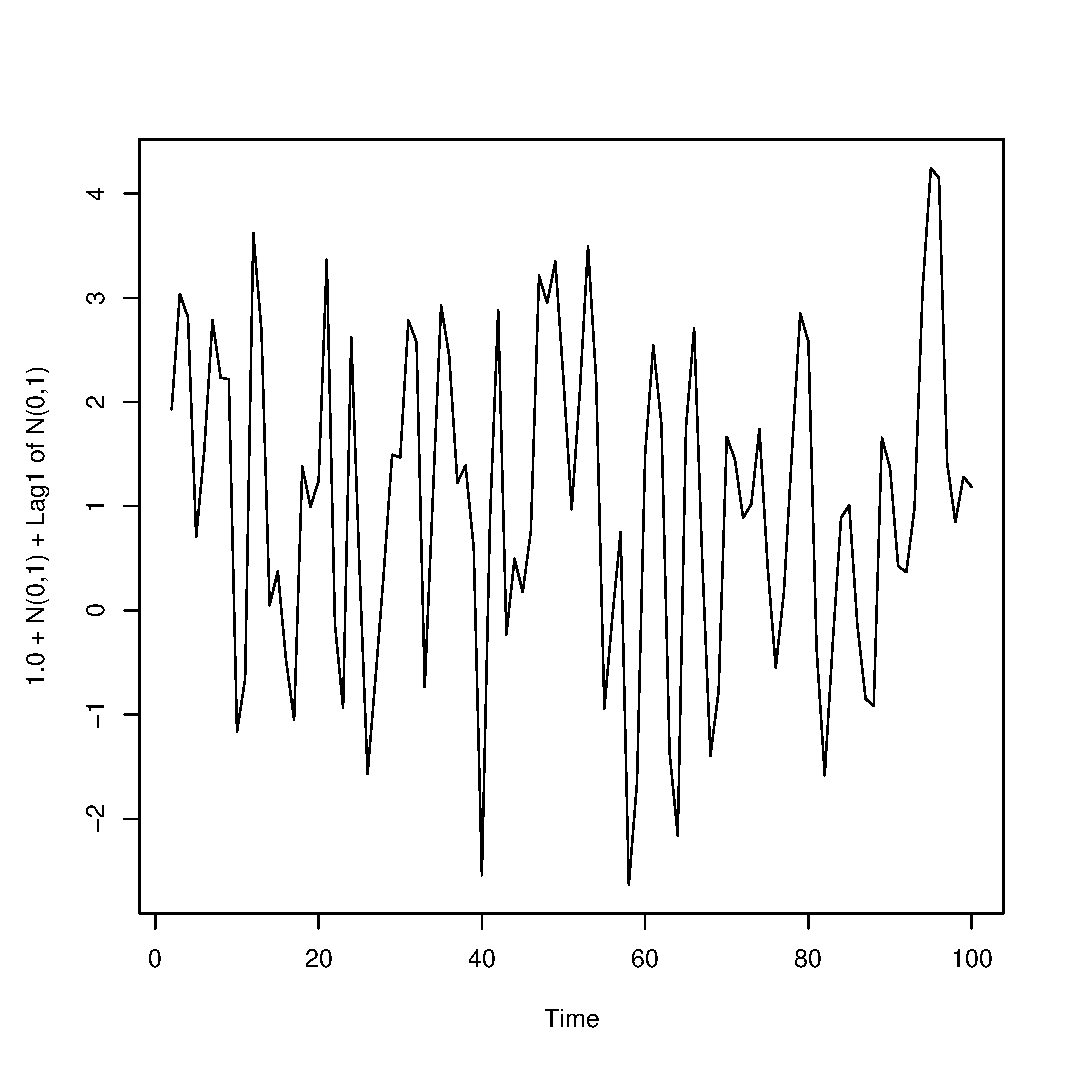
\includegraphics[scale=0.26]{chapters/chapter_uvts/figures/ch1fig1y2ts.eps}
                        }
                        \hfill
                \subfloat[Figure 1e]
                        [ACF]
                        {
                        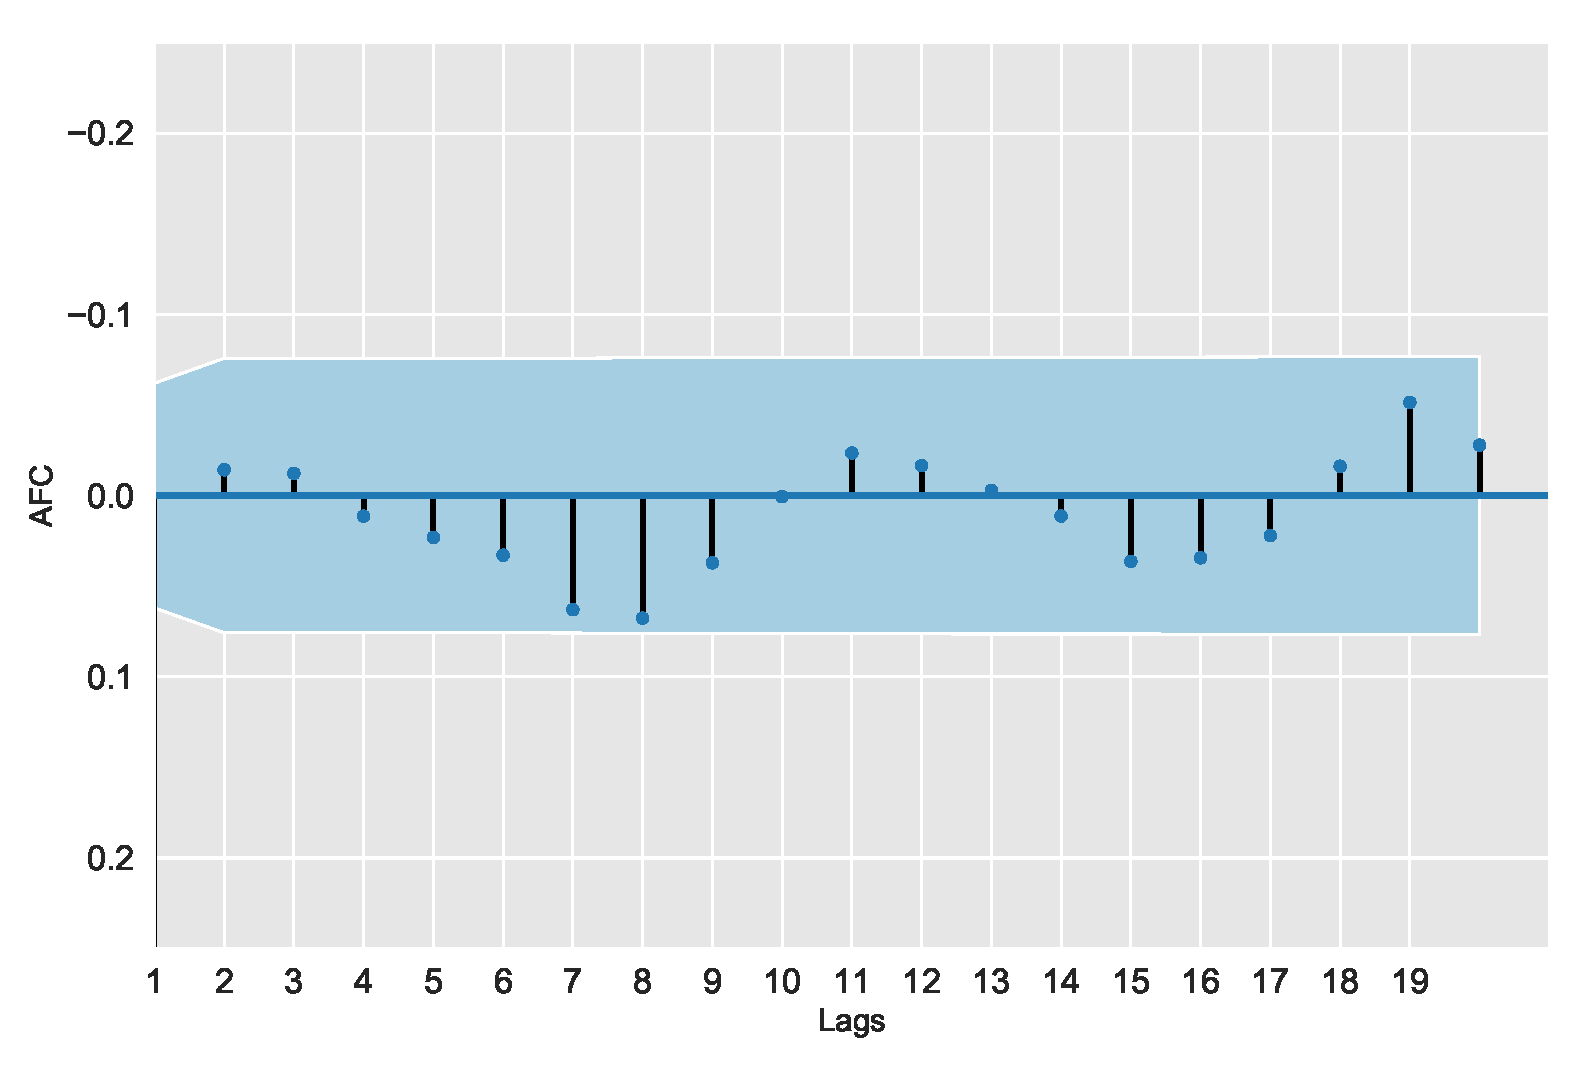
\includegraphics[scale=0.26]{chapters/chapter_uvts/figures/ch1fig1y2acf.eps}
                        }
                        \hfill
                \subfloat[Figure 1f]
                        [$Y_t$ vs. $Y_{t-1}$]
                        {
                        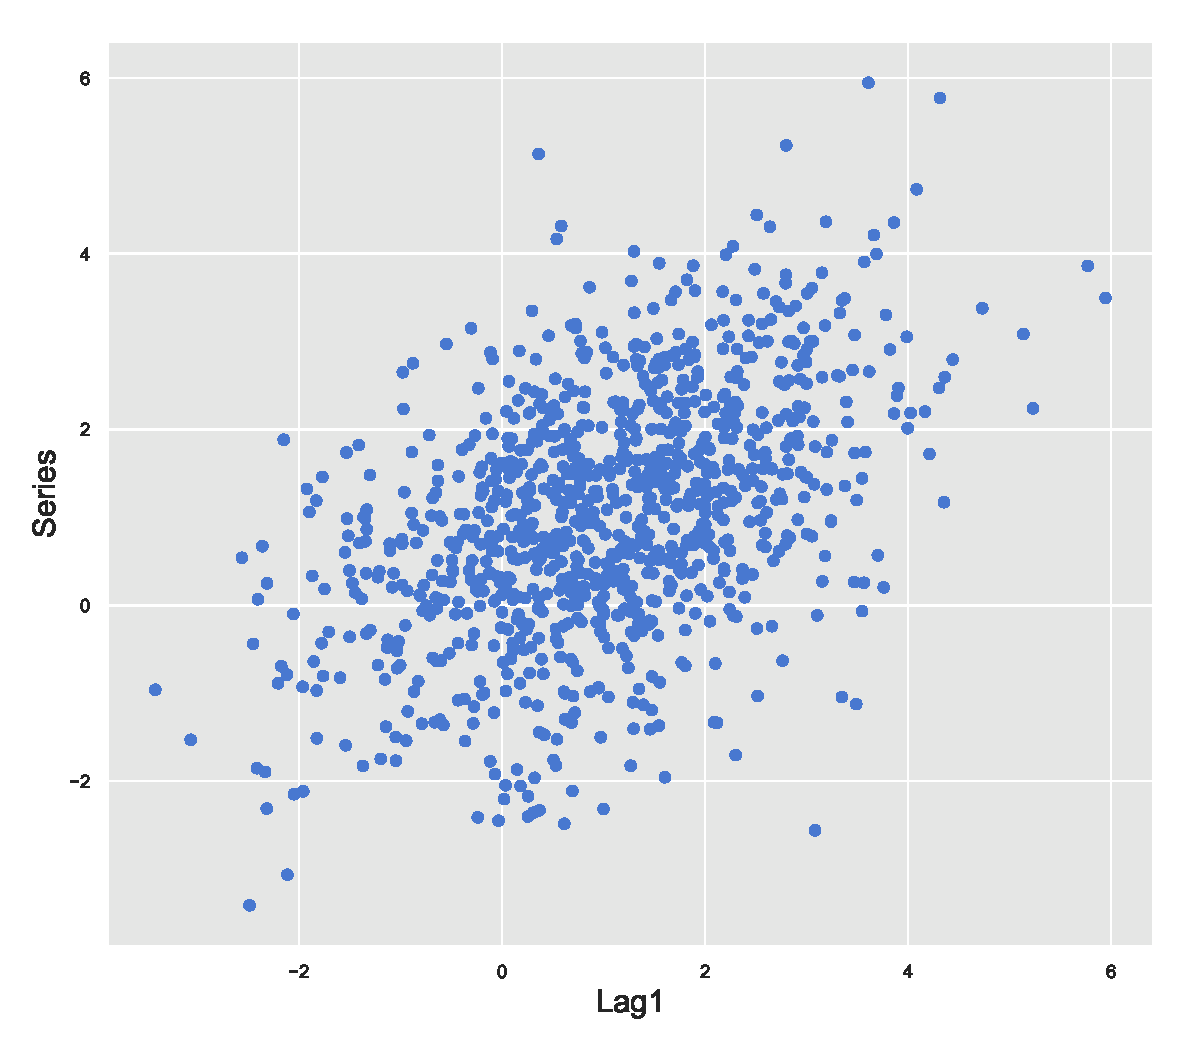
\includegraphics[scale=0.26]{chapters/chapter_uvts/figures/ch1fig1y2lagplot.eps}
                        }
               \caption{Processes \& Diagnostics from $Y_t = 0.5 + \epsilon_t$ and from $Y_t = 1.0 + \epsilon_t + \epsilon_{t-1}$. \label{fig:sideways}}
            \end{sidewaysfigure}


Figure~\ref{fig:sideways}~(a) shows a time series plot of a computer simulated series of 100 values from a Gaussian white noise process $\{ \epsilon_t \}$ with $\sigma^2= 1$, while Figure~\ref{fig:sideways}~(b) shows a plot of the corresponding values of the series $Y_t = 1.0 + \epsilon_{t} + \epsilon_{t-1}$ using these same $\{\epsilon_t\}$.  Note the relatively much smoother behavior over time of the data in (b) than in (a), due to the positive autocorrelation at lag one of the process in (b) which tends to make successive values of the series behave more similarly to each other.  Similar to Example~\ref{ex:movingaverage}, it is easy to show that the process $\{Y_t\}$ defined by the relation $Y_t = \mu + \epsilon_{t} - \epsilon_{t-1}$ is stationary with autocorrelation function $\rho(0)=1$, $\rho(1)=-1/2$, and $\rho(s)=0$ for $|s|>1$. A plot of a simulated series from this process is given in Figure~\ref{fig:sideways}~(d) which shows the much ``rougher'' or less smooth behavior over time relative to the behavior  in (a) and (b) due to the addition of extra noise to the model. These figures form the basis of model building and the subsequent diagnostic checks on the fitness of models. \xqed
\end{ex} 


\noindent \textbf{Examples of Nonstationary Stochastic Processes} \\


Many time series that occur in finance do not exhibit stationary behavior.  For example, stock price series show a trend or change in the mean level over time, reflecting information flow about the stock or investors' behavior. Series also exhibit seasonal behavior, either in the form of nonstationary or deterministic seasonal patterns, both of which need to be distinguished from purely nondeterministic stationary stochastic behavior. Other departures from stationarity include changes in variability of the process over time (nonconstant variance or volatility regimes), abrupt shifts in the mean level, and changes in the autocorrelation structure of the process over time which is a feature of the series which would typically be more difficult to detect.  An important practical matter in the analysis of time series data involves methods of transforming a nonstationary time series into a stationary series, and accounting for and modeling of the nonstationary aspects of the original series. Many of the methods that are found useful in practice involve considering successive changes or differences over time in the original series to remove the nonstationary features of the series, especially changes in the mean level, or using linear regression techniques to help account for the nonstationary mean behavior.  We will illustrate this with a few simple but commonly occurring examples. 


\begin{ex}[Random Walk with a Drift] \label{ex:driftwalk} 
Let $\{ \epsilon_t, \, t=0,1,2, \ldots \}$ be a sequence of independent random variables with mean 0 and variance $\sigma^2$, and define a new process $\{ Y_t \}$ recursively by
	\[
	Y_t = Y_{t-1} + \delta + \epsilon_t, \qquad t=0,1,2, \ldots, \quad Y_0 = 0,
	\]
where $\delta$ is a constant.  By successive substitutions in the above relations for $Y_t$, we find that $\{Y_t\}$ can also be expressed as
	\[
	Y_t = \delta \, t + \sum_{j=1}^t \epsilon_j = \delta \, t + \epsilon_{t} + \epsilon_{t-1} + \cdots + \epsilon_{1}, \qquad t= 1, 2, \ldots .
	\]
Hence we see that $E(Y_t)= \delta t$ and $\var(Y_t)= \var(\sum_{j=1}^t \epsilon_j)= \sum_{j=1}^t \var(\epsilon_j)= t \, \sigma^2$, so that the process $\{ Y_t \}$ is not stationary and exhibits change in both mean and variance.  Moreover, for any $s > 0$, we find that
	\[
	\cov(Y_t,Y_{t+s})= \cov \left( \sum_{j=1}^t \epsilon_j, \sum_{i=1}^{t+s} \epsilon_i \right)= \sum_{j=1}^t \var(\epsilon_j) = t \, \sigma^2 ,
	\]
so that $\corr(Y_t,Y_{t + s}) = t / \sqrt{t(t + s)} = 1/ \sqrt{1 + s/t}$. Note that this correlation is close to one for large $t$ and relatively small $s$, so that nearby values $Y_t$ and $Y_{t+s}$ of the process $\{Y_t\}$ are highly positively correlated.  However, note that the time series of \emph{first differences} of the process $\{ Y_t \}$, defined by $Z_{t}=Y_{t}-Y_{t-1}$, forms a stationary process, because $Z_{t}= Y_{t} - Y_{t-1} = \delta + \epsilon_t$, a white noise series as in Example~\ref{ex:whitenoise}. Such a process $\{ Y_t \}$ whose first differences form a white noise series, is called a random walk process with a drift. Time series plots of simulated data from random walk exhibit behavior with little tendency to vary around a fixed constant mean level. The parameter $\delta$ in the random walk model is referred to as the drift in the random walk process. Note the trend behavior in the process with $\delta > 0$. \xqed
\end{ex}


Of course, a more general class of models is obtained by supposing that a nonstationary process $\{ Y_t \}$ is such that its first differences form a stationary process, but not necessarily white noise.  It has been found from practical experience that this type of model is quite useful in producing adequate representations for actual observed financial series in many cases.



% Some Basic Models and Descriptive Tools
\subsection{Some Basic Models and Descriptive Tools} 


Suppose we have a sample realization of $T$ observations $Y_1, Y_2, \ldots, Y_T$ from a stationary process $\{Y_t\}$ which has a mean $\mu=E(Y_t)$, autocovariance function (ACF) $\gamma(s)= \cov(Y_t,Y_{t+s})$ and autocorrelation function $\rho(s)= \corr(Y_t,Y_{t+s}) = \gamma(s)/\gamma(0)$. Because the ACF $\rho(s)$ is such a basic quantity that describes the correlation properties of the process, we are naturally interested in obtaining estimates of $\rho(s)$ from the sample data.


First, a natural estimator of $\mu$ is the sample mean $\overline{Y}= (1/T) \sum_{t=1}^T Y_t$. The most common estimator used for $\gamma(s)$ is the sample autocovariance function defined by
	\[
	\hat{\gamma}(s)= \frac{1}{T} \sum_{t=1}^{T-s} \, \left(Y_{t}-\overline{Y}\right) \left(Y_{t+s}-\overline{Y}\right), \quad s=0, 1, \ldots.
	\]
Usually one only computes $\hat{\gamma}(s)$ for lags $s$ much smaller than $T$, say, $0 \leq s \leq T/4$, since $\hat{\gamma}(s)$ for large lags are typically not very informative or of much interest. Note that $\hat{\gamma}(s)$ has the form of an ordinary sample covariance between the pairs of variables $(Y_t, Y_{t+s})$, except for the use of the common sample mean $\overline{Y}$ for both variables and the divisor $T$ in place of $T-s$.  Note also that $\hat{\gamma}(0) = T^{-1}\sum_{t=1}^T (Y_t-\overline{Y})^2$ represents the sample variance of the data.  The estimator of $\rho(s)$ follows directly from $\hat{\gamma}(s)$ and is given by
	\begin{equation} \label{eqn:hatrho}
         \hat{\rho}(s)= \frac{\hat{\gamma}(s)}{\hat{\gamma}(0)}= \frac{\sum_{t=1}^{T-s} \left(Y_{t}-\overline{Y}\right) \left(Y_{t+s}-\overline{Y}\right)}{\sum_{t=1}^T(Y_t-\overline{Y})^2} , \quad s= 0, 1, \ldots,
	\end{equation}
which is called the sample ACF.  The sample ACF will also sometimes be denoted as $\hat{\rho}(s) \equiv r(s)$.


We now briefly discuss a few properties of the sampling distributions of the above estimators, with particular emphasis on the sample ACF $r(s)$.  The mean of $\overline{Y}$ is easily seen to be $E(\overline{Y})= (1/T) \sum_{t=1}^T E(Y_t) = \mu$, so that $\overline{Y}$ is an unbiased estimator of $\mu$.  The variance of $\overline{Y}$ is
	\begin{equation} \label{eqn:var}
        \var(\overline{Y})= \frac{\gamma(0)}{T} \left[ 1 + 2 \sum_{u=1}^{T-1} \frac{T - u}{T} \rho(u) \right].
        \end{equation}
Hence if $\rho(u) \rightarrow 0$ as $u \rightarrow \infty$, then so that $\var\left(\overline{Y}\right) \rightarrow 0$ as $T \rightarrow \infty$. Under some mild conditions it can also be shown that $\overline{Y}$ is asymptotically normally distributed as $T \rightarrow \infty$.


The sampling properties of the sample ACF $r(s)$ are quite complicated and exact results are not available except in a few special cases. We indicate one result from Anderson and Walker (1964)~\cite{anderwalk} based on large sample theory. Under linearity of the time series, the joint distribution of $\big(T^{1/2} (r(1) - \rho(1) ), \ldots, T^{1/2} (r(k) - \rho(k) ) \big)$, $k$ fixed, tends to follow a multivariate normal $N(0, W)$ distribution as $T \to \infty$, where $W$ is a $k \times k$ matrix with $(i,j)$th element, $w_{ij}$, given by
	\begin{equation} \label{eqn:wij}
	\begin{split}
	w_{ij}= \sum_{\nu= -\infty}^\infty & [\, \rho(\nu + i ) \rho(\nu + j) + \rho(\nu - i) \rho(\nu + j) - 2 \rho(\nu) \rho(j) \rho(\nu + i)  \\
	&- 2 \rho(\nu) \rho(i) \rho(\nu + j) + 2 \rho(\nu)^2 \rho(i) \rho(j)], \quad  i, j= 1,\ldots, k.
        \end{split}
	\end{equation}
Hence for large $T$, we have the approximations $E(r(s)) \approx \rho(s)$, $\var(r(s)) \approx w_{ss}/T$, $\cov(r(s), r(u)) \approx w_{su}/T$, and the $r(s)$ are approximately normally distributed. The equation \eqref{eqn:wij} is also called Bartlett's formula and dates back to 1946.


There are a few special cases of \eqref{eqn:wij} worth noting. In the white noise case where the $Y_t$ are independent r.v.'s, we then have $\rho(\nu)= 0$ for all $\nu \neq 0$ and so the approximations reduce to $E(r(s)) \approx 0$, $\var(r(s)) \approx 1/T$, $\cov(r(s), r(u)) \approx 0$, or more exactly, $\var(r(s)) \approx (T-s)/T^2$. Hence we can use these results to check for ``non-randomness'' of a series of comparing the sample values $r(s)$ at various lags $s=1, \ldots, k$ with the approximate 95\% limits $\pm \, 2 \sqrt{(T-s)/T^2} \approx 2 / \sqrt{T}$ for the normal distribution to see whether the $r(s)$ generally fall within these limits. We will use this test repeatedly on the residuals as a diagnostic tool for model adequacy. 


In the second case, suppose it is assumed that the theoretical ACF satisfies $\rho(\nu) = 0$ for all $|\nu| > q$.  Then, for any $s > q$ the expression for the approximate variance of $r(s)$ reduces to
	\begin{equation} \label{eqn:varrs}
	\var(r(s)) \approx \dfrac{1}{T} \sum_{\nu=-q}^q \rho(\nu)^2= \dfrac{1}{T} \left[ 1 + 2 \sum_{\nu=1}^q \rho(\nu)^2 \right], \quad s > q 
	\end{equation}        
and
	\[
	\cov(r(s), r(u)) \approx \frac{1}{T} \sum_{\nu = -q}^{q} \rho(\nu)\, \rho(\nu - s + u), \quad s,u > q.
	 \]

As one final special case, suppose the process  has ACF of the simple form (which results from an autoregressive model of order one (AR(1)), with coefficient $\phi$) $\rho(\nu) = \phi^{|\nu|}$, $\nu= 0, \pm 1, \ldots$, with $|\phi| < 1$. Then
	\[
	\var(r(s)) \approx \frac{1}{T} \left[ \frac{(1 + \phi^2) (1 - \phi^{2s})}{1 - \phi^2} - 2s \phi^{2s} \right],
	\]
and in particular $\var(r(1)) \approx \frac{1}{T} (1 - \phi^2)$.


The plot of ACF for a white noise sequence for a large number of lags may have a few isolated lags lie outside the limits, $\pm \frac{2}{\sqrt{T}}$. But characteristic behavior of nonstationary series is that the sample ACF values $r(s)$ are slow to ``dampen out'' as the lag $s$ increases. \\


\noindent\textbf{Linear Models for Stationary Time Series} \\


A stochastic process $\{ Y_t \}$ will be called a \emph{linear process} if it can be represented as
	\begin{equation} \label{eqn:yt}
          Y_t = \mu + \sum_{j=0}^{\infty}  \psi_j \epsilon_{t-j},
	\end{equation}
where the $\epsilon_t$ are independent with 0 mean and variance $\sigma^2_{\epsilon}$, and $\sum_{j=0}^{-\infty} \lvert \psi_j \rvert < \infty$. This process may also be referred to as an infinite moving average process.


We now introduce, for notational convenience, the backward shift operator $B$, defined by the property that $B^j Y_t = Y_{t-j}$ for any time series $\{ Y_t \}$. Model~\eqref{eqn:yt} may be expressed as
	\[
	Y_t = \mu + \sum_{j=0}^{\infty} \psi_j B^j \epsilon_t = \mu + \psi(B) \epsilon_t,
	\]
where $\psi(B) = \psi_0 + \psi_1 \, B + \psi_2 \, B^2 + \cdots$ is referred to as the infinite moving average operator. Since the input $\{\epsilon_t\}$ is a stationary process, it follows that $\{ Y_t \}$ in \eqref{eqn:yt} forms a stationary process, with mean $E(Y_t)=\mu$ and autocovariance function
	\begin{equation} \label{eqn:covyt}
	\gamma(s)= \cov(Y_t, Y_{t+s})= \sigma^2_{\epsilon} \sum_{j=0}^{\infty} \psi_j \psi_{j+s},
	\end{equation}      
because $\gamma_\epsilon(s) = \sigma^2_\epsilon$ if $s=0$ and $\gamma_\epsilon(s) = 0$ if $s \neq 0$, so that $\gamma_\epsilon(j - k + s) = 0$ when $k \neq j = s$.
	

An important result called Wold's Theorem indicates the generality of the class of linear processes in stationary theory, that every purely non-deterministic stationary process may be expressed in an infinite moving average representation as in \eqref{eqn:yt}, although the $\epsilon_t$ need not be independent but merely uncorrelated.	


The general linear representation model given by \eqref{eqn:yt} although useful for studying the properties of time series models but is not directly useful in practice to represent a stationary process, since it requires the determination of an infinite number of unknown parameters $\psi_1, \psi_2, \ldots$, from a finite record of data. Hence we now consider finite parameter models of the same type which will be useful representations and are sufficiently general to well approximate the model for any process of the form \eqref{eqn:yt}. \\


\noindent \textbf{Finite Moving Average Processes} \\


A direct way to obtain finite parameter models from the general form \eqref{eqn:yt} is simply to restrict the $\psi_j$ to be zero beyond some lag $q$. Thus (with a change of notation), a stationary process $\{ Y_t \}$ is said to be a \emph{moving average process} of order $q$, which is denoted as MA($q$), if it satisfies
	\begin{equation} \label{eqn:yt2}
	Y_t = \mu + \epsilon_t - \sum_{j=1}^{q} \theta_j \epsilon_{t-j},
	\end{equation}
where the $\epsilon_t$ are independent with mean 0 and variance $\sigma^2$. Using the backward shift operator notation $B$, the MA($q$) model can be expressed as
	\begin{equation*}
         Y_t= \mu + \theta(B) \, \epsilon_t,	
	\end{equation*}
where $\theta(B) = 1 - \sum_{j=1}^q \theta_j B^j$.  An MA($q$)  process is always stationary, by Theorem~\ref{thm:wold}, because $\sum_{j=0}^{\infty} \lvert \psi_j \rvert= 1 + \sum_{j=1}^q \lvert \theta_j \rvert$ is always finite. The mean of the process is $\mu = E(Y_t)$, and the autocovariance function is (from \eqref{eqn:covyt})
	\begin{equation*}
            \gamma(s)= \cov (Y_t, Y_{t+s})= \sigma^2 \sum_{j=0}^{q-s} \theta_j \theta_{j+s}, \quad s = 0, 1, 2, \ldots, q,	
	\end{equation*}
and $\gamma(s)= 0$ for $s > q$, where $\theta_0$ is defined to be $-1$. So in particular, $\gamma(0)=  \var(Y_t) = \sigma^2 (1 + \sum_{j=1}^q \theta_j^2)$. Hence the autocorrelation function of an MA($q$) process \eqref{eqn:yt2} is
       \begin{equation} \label{eqn:rhos}
	\rho(s) = \dfrac{-\theta_s + \sum_{j=1}^{q-s} \theta_j \theta_{j+s}}{1 + \sum_{j=1}^q \theta_j^2}, \quad s = 0,1,\ldots, q
       \end{equation}
and $\rho(s)= 0$ for $s > q$. The prominent feature of the ACF of an MA($q$) process is that it equals zero or ``cuts off'' after a finite number of lags, $q$. Thus in one sense the ``memory'' of an MA($q$) process is $q$ periods long. In practice, useful MA($q$) models are those for which the value of $q$ is typically quite small, such as $q= 1, 2,$ or $3$.  For financial time series, usually $q= 1$ will suffice for modeling, which we will discuss below. 


\begin{ex}[Moving Average Model of Order 1 (MA(1))] \label{ex:movingorder1}
The simplest example of a moving average process is that of order one, MA(1), given by
	\[
	Y_t = \mu + \epsilon_t - \theta \epsilon_{t-1}= \mu + (1 - \theta B) \epsilon_t.
	 \]
Its autocovariances are $\gamma(0)= \sigma^2 (1 + \theta^2)$, $\gamma(1)= -\theta\, \sigma^2$, and $\gamma(s)= 0$ for $s > 1$, and hence the ACF is $\rho(1)= -\theta / (1+\theta^2)$, $\rho(s)= 0$, $s > 1$. It is easy to show that the largest possible value of $\left| \rho(1) \right|= \left| \theta \right| / (1+\theta^2)$ for an  MA(1) process is $\rho(1)= \pm 0.5$ which occurs when $\theta = \pm 1$. This illustrates that in general there are further restrictions on the autocorrelation function $\rho(s)$ of an MA($q$)  process in addition to $\rho(s)= 0, s > q$. \xqed
\end{ex}
    

\begin{ex}[Seasonal Moving Average] \label{ex:seasonal} 
For time series which may exhibit seasonal correlation, such as certain financial time series with week-day effect, the following type of special seasonal moving average (SMA) model is useful. Let $S$ denote the number of discrete time periods per seasonal period (for example, $S= 4$ for quarterly data of an annual seasonal nature), and define the process $\{ W_t \}$ by
	\[	
	W_t = \mu + \epsilon_t - \tau_S \, \epsilon_{t-S}.
	\]
Then we find that $\gamma(0)= \sigma^2 (1+\tau_S^2)$, $\gamma(S) = - \tau_S / (1+\tau_S^2)$,  and $\rho(j)= 0$ for all $j \neq 0, \pm S$. Hence this process exhibits nonzero autocorrelation only at the seasonal lag $S$. This model is known as a SMA model of seasonal order 1 (and period $S$), and its generalizations are useful when modeling seasonal differences $W_t = Y_t - Y_{t-S}$ of an original seasonal time series $\{ Y_t \}$.  In the context of financial data, this could be used to model the so called Monday and Friday effects on price and volatility. \xqed
\end{ex}      


\begin{ex}[Autoregressive Model of Order 1 (AR(1))] \label{ex:autoregor1}
Consider the process \eqref{eqn:yt} with coefficients given by $\psi_j = \phi^j$, $j= 0,1,\ldots$,  for some $\phi$ with $\lvert \phi \rvert < 1$. Then the process $Y_t = \mu + \sum_{j=0}^{\infty} \phi^j \epsilon_{t-j}$ is stationary, because $\sum_{j=0}^{\infty} \lvert \psi_j \rvert= \sum_{j=0}^{\infty} \lvert \phi \rvert^j = 1/(1 - \lvert \phi \rvert)$ is absolutely convergent for $\lvert \phi \rvert < 1$. From \eqref{eqn:covyt}, the autocovariance function of $\{ Y_t \}$ is
	\[
	\gamma(s)= \sigma^2_{\epsilon} \sum_{j=0}^{\infty} \phi^j \phi^{j+s}= \sigma^2_{\epsilon} \phi^s \sum_{j=0}^{\infty} \phi^{2j}= \frac{\sigma^2_{\epsilon} \phi^s}{1 - \phi^2}, \quad s \geq 0.
	\]
In particular, $\gamma(0) = \var(Y_t) = \sigma^2_{\epsilon}/(1-\phi^2)$. Hence the autocorrelation function of $\{ Y_t \}$ is $\rho(s)= \gamma(s) / \gamma(0)= \phi^s$, $ s \geq 0$ which declines exponentially (geometrically) as the lag $s$ increases.


Note that the process $\{Y_t\}$ defined above actually satisfies the relation 
	\[
	Y_t= \phi \, Y_{t-1} + \delta+\epsilon_t,
	\]
$t= \ldots ,-1, 0, 1, \ldots$, with $\delta = \mu(1 - \phi)$. This process is called a first-order autoregressive process, and is a special case of the general class of autoregressive processes which is discussed below. Also note that if the value of $\phi$ in the above is taken as  $\phi = 1$, then the arguments for stationarity of $\{Y_t\}$ no longer hold, because $\sum_{j=0}^{\infty} \lvert \psi_j \rvert = 1 + 1 + \cdots$ does not converge. We see that in this case the process is actually a (nonstationary) random walk satisfying the relation  $Y_t = Y_{t-1} + \epsilon_t$, a common representation of the behavior of the stock prices under the efficient market hypothesis. \xqed
\end{ex}


\noindent\textbf{General Order Autoregressive Processes} \\


While stock price data exhibit simpler structures such as AR(1) in daily aggregation and MA(1) in smaller time unit aggregation such as five minutes, the volume of trading is shown to have more complex dependencies. The behavior of volume and other trade related data are best captured by higher order ARMA models. 

Consider the AR($p$) process $\{ Y_t \}$ defined by
	\begin{equation} \label{eqn:ytsum}
	Y_t = \phi_1 Y_{t-1} + \phi_2 Y_{t-2} + \cdots + \phi_p Y_{t-p} + \delta + \varepsilon_t
	\end{equation}
or $(1 - \phi_1 B - \phi_2 B^2 - \cdots - \phi_p B^p) Y_t = \delta + \varepsilon_t$. When $p= 1, Y_t = \phi Y_{t-1} + \delta + \varepsilon_t$, the ACF, $\rho(v)= \phi^{\lvert \nu \rvert}$ takes the simple form, as observed earlier.


\begin{result}
If the roots of $\phi(z) = 1- \phi_1 z - \cdots - \phi_p z^p = 0$ are greater than one in absolute value, then $\{ Y_t \}$ defined by \eqref{eqn:ytsum} is a stationary AR($p$) process and has a convergent one-sided infinite moving average representation as
	\begin{equation} \label{eqn:ytthm}
	Y_t= \mu + \sum_{j=0}^\infty \Psi_j\varepsilon_{t-j},
	\end{equation}
where $\mu = E(Y_t) = \delta / (1 - \phi_1 - \cdots - \phi_p)$, $\Psi(B) = \sum_{j=0}^\infty \Psi_j B^j$. 
\end{result}


The autocovariance $\gamma(s)$ for the AR($p$) process satisfy the \emph{Yule-Walker equations} given by
	\begin{equation*}
	\gamma(s)= \cov(Y_t,Y_{t-s}) = \phi_1 \gamma(s-1) + \phi_2 \gamma(s-2) + \cdots + \phi_p \gamma(s-p), \quad s= 1,2,\ldots,
	\end{equation*}
noting again that $\cov(\varepsilon_t,Y_{t-s})= 0$, for $s > 0$. Dividing by $\gamma(0)$, the ACF $\rho(s)$ also satisfies the relations
	\begin{equation} \label{eqn:rhos2}
	\rho(s) = \phi_1 \rho(s-1) + \phi_2 \rho(s-2) + \cdots + \phi_p \rho(s-p), \quad s= 1,2,\ldots.
	\end{equation}
The Yule-Walker equations \eqref{eqn:rhos2} for $s= 1, 2, \ldots, p$ are particularly useful for determining the autoregressive parameters $\phi_1, \ldots, \phi_p$ in terms of the autocorrelations. Note that these equations can be expressed in matrix form as $P_p \phi = \rho$, where
	\begin{equation} \label{eqn:matrix}
	P_p = 
	\begin{bmatrix}
	1 & \rho(1) & \rho(2) & \cdots & \rho(p-1) \\
	\rho(1) & 1 & \rho(1) & \cdots & \rho(p-2)\\
	\vdots & & \ddots & & \vdots \\
	\rho(p-1) & \cdots & & \rho(1) & 1
	\end{bmatrix}, \quad
	\phi= \begin{bmatrix} \phi_1 \\ \phi_2 \\ \vdots \\ \phi_p \end{bmatrix}, \quad
	\rho= \begin{bmatrix} \rho(1) \\ \rho(2) \\ \vdots \\ \rho(p) \end{bmatrix}.
	\end{equation}
These equations can be used to solve for $\phi_1, \ldots, \phi_p$ in terms of $\rho(1), \ldots, \rho(p)$, with solution $\phi = P_p^{-1} \rho$. Note also, that the variance of the process, $\gamma(0) = \var(Y_t)$, and $\sigma^2= \var(\varepsilon)$, are related by
	\begin{equation} \label{eqn:gamma0cov}
	\gamma(0)= \cov(Y_t, \phi_1 Y_{t-1} + \cdots + \phi_p Y_{t-p} + \delta + \varepsilon_t)= \phi_1 \gamma(1) + \cdots + \phi_p \gamma(p) + \sigma^2,
	\end{equation}
because $\cov(Y_t, \varepsilon_t)= \sigma^2$. Hence $\sigma^2$ can be determined in terms of $\gamma(0)$ and the autocorrelations $\rho(s)$ from \eqref{eqn:gamma0cov}.


Also note that a measure of the strength of association or ``predictability'' of $Y_t$ based on its past values $Y_{t-1}, \ldots, Y_{t-p}$ can be given by the (squared) multiple correlation coefficients of $Y_t$ with $(Y_{t-1}, \ldots, Y_{t-p})$, which is $R^2= (\gamma(0) - \sigma^2)/\gamma(0) = 1 - ( \sigma^2 / \gamma(0) ) = \phi_1 \rho(1) + \cdots + \phi_p \rho(p)$. Since $\gamma(0)$ represents the ``total'' variance of $Y_t$, and $\sigma^2$ may be interpreted as the ``unexplained'' or error variance (i.e., that portion of the variance not explained by the past values), the quantity $R^2$ has the usual interpretation as in linear regression of representing the proportion of the total variance of the variable $Y_t$ that is explained by (auto)regression on the past values $Y_{t-1}, \ldots, Y_{t-p}$. \\


\noindent\textbf{Partial Autocorrelation Function} \\


When an AR model is being fit to observed time series data, the sample version of the Yule-Walker equations \eqref{eqn:rhos2}, \eqref{eqn:matrix}, in which the values $\rho(j)$ are replaced by the sample ACF values r(j), can be solved to obtain estimates $\hat{\phi}_j$ of the autoregressive parameters. However, initially it is not known which order $p$ is appropriate to fit to the data. The sample partial autocorrelation function (PACF) will be seen to be useful for determination of the appropriate order of an AR process as how the autocorrelation function (ACF) is useful for the determination of the appropriate order of an MA process. First, we discuss the concept of PACF in general.


Suppose $\{ Y_t \}$ is a stationary process, not necessarily an AR process, with ACF $\rho(j)$. For general $k \geq 1$, consider the first $k$ Yule-Walker equations for the ACF associated with an AR($k$) process.
	\begin{equation} \label{eqn:rhoj}
	\rho(j) = \phi_1 \rho(j-1) + \phi_2 \rho(j-2) + \cdots + \phi_k \rho(j-k), \quad j = 1, 2,\ldots, k
	\end{equation}
and let $\phi_{1k}, \phi_{2k}, \ldots, \phi_{kk}$ denote the solution for $\phi_1, \phi_2, \ldots, \phi_k$ to these equations. Given the ACF $\rho(j)$, \eqref{eqn:rhoj} can be solved for each value $k= 1,2, \ldots$, and the quantity $\phi_{kk}$, regarded as a function of the lag $k$, is called the (theoretical) \emph{partial autocorrelation function} (PACF) of the process $\{ Y_t \}$. The values $\phi_{1k},  \phi_{2k}, \ldots, \phi_{kk}$ which are the solution to \eqref{eqn:rhoj} are the regression coefficients in the regression of $Y_t$ on $Y_{t-1}, \ldots, Y_{t-k}$; that is, values of coefficients $b_1, \ldots, b_k$ which minimize $E[(Y_t - b_0 - \sum_{i=1}^k b_iY_{t-i})^2]$.


If $\{ Y_t \}$ is truly an AR process of order $p$, the $\phi_{kk}$ will generally be nonzero for $k \leq p$, but $\phi_{kk}$ will always be zero for $k > p$. This is so since the ACF $\rho(j)$ actually satisfies the Yule-Walker equations \eqref{eqn:rhoj} for $k= p$, and hence for any $k > p$ the solution to \eqref{eqn:rhoj} must be $\phi_{kk}= \phi_1, \ldots, \phi_{pk}= \phi_p$, $\phi_{p+1,k} = 0, \ldots,\phi_{kk} = 0$, where $\phi_1, \ldots, \phi_p$ are the true AR coefficients. Thus, the PACF $\phi_{kk}$ of an AR($p$) process ``cuts off'' (is zero) after lag $p$, and this property serves to distinguish (identify) an AR($p$) process.


The quantity $\phi_{kk}$ defined above is called the \emph{partial autocorrelation} at lag $k$, since it is actually equal to the partial correlation between the r.v.'s $Y_t$ and $Y_{t-k}$ adjusted for the intermediate variables $Y_{t-1}, Y_{t-2}, \ldots, Y_{t-k+1}$, and $\phi_{kk}$ measures the correlation between $Y_t$ and $Y_{t-k}$ after adjusting for the effects of $Y_{t-1}, Y_{t-2}, \ldots, Y_{t-k+1}$.


Based on a sample $Y_1, \ldots, Y_T$ from a process $\{ Y_t \}$, the sample PACF value at lag $k$, $\hat{\phi}_{kk}$, is obtained as the solution to the sample Yule-Walker equations of order $k$,
	\begin{equation} \label{eqn:rjequation}
	r(j) = \hat{\phi}_{tk} r(j-1) + \cdots + \hat{\phi}_{kk} r(j-k), \quad j = 1, \ldots ,k,
	\end{equation}
for each $k= 1, 2, \ldots$. These are the same form as the equations \eqref{eqn:rhoj} but with sample ACF values $r(j)$ used in place of the theoretical ACF values $\rho(j)$. In matrix notation similar to that used in \eqref{eqn:matrix}, the solution is $\hat{\phi} = R_k^{-1} r$. Now under the assumption that the process $\{ Y_t \}$ is an AR of order $p$, the estimated PACF values $\hat{\phi}_{kk}$ for lags $k > p$ are approximately independently and normally distributed for large $T$, with mean $E(\hat{\phi}_{kk})= 0$ and St.Dev. $\hat{\phi}_{kk} = 1 / \sqrt{T}$ for $k > p$. These facts concerning the sampling properties of the sample PACF $\hat{\phi}_{kk}$ can be used to assess whether the coefficients in estimated AR models may be treated as close to zero after some lag $p$ (e.g. if $\lvert \hat{\phi}_{kk} \rvert < 2 / \sqrt{T}$ for $k > p$), and hence can be useful in the selection of an appropriate order $p$ for fitting an AR model to sample data. \\


\noindent\textbf{Linear Models for Nonstationary Time Series} \\


Often, in practice, series $\{ Y_t \}$ will be encountered which are nonstationary. One type of nonstationary series that occurs commonly, are series that exhibit some homogeneous behavior over time in the sense that, except for local level or perhaps local level and local trend, one segment of the series behaves much like any other part of the series. In cases where the series $\{ Y_t \}$ exhibits such homogeneous nonstationarity, it may be found that the first difference of the series, $(1 - B)\, Y_t = Y_t - Y_{t-1}$, is a stationary series. For seasonal nonstationary time series that exhibit homogeneous behavior apart from a seasonal mean level or trend, with seasonal period $S$, the seasonal difference of the series, $(1 - B^s)\, Y_t = Y_t - Y_{t-s}$, may be stationary. More generally, a useful class of models for this type of homogeneous nonstationary time series $\{Y_t\}$ is obtained by assuming that the $d$th difference, $W_t = (1 - B)^d\,Y_t$, is a stationary series, and $W_t$ can be represented by an ARMA($p,q$) model. The most common case is $d=1$, for financial time series. \\


\noindent\textbf{Autoregressive Integrated Moving Average Processes (ARIMA)} \\


We consider models for $\{ Y_t \}$ such that $W_t = (1 - B)^d\, Y_t$ is a stationary ARMA$(p,q)$ process. The process $\{ Y_t \}$ is then said to be an \emph{autoregressive integrated moving average process} of order $(p,d,q)$, denoted as ARIMA$(p,d,q)$. Since the $d$th differences $W_t$ form an ARMA$(p,q)$ process, they satisfy $\phi(B)\, W_t = \delta + \theta(B)\, \varepsilon_t$. So the ARIMA process $Y_t$ is generated by 
	\begin{equation} \label{eqn:phiBdy}
	\phi(B)(1 - B)^d\, Y_t = \delta + \theta(B)\varepsilon_t,
	\end{equation}
where $\phi(B) = 1 - \phi_1 B - \cdots - \phi_p B^p$ and $\theta(B) = 1 - \theta_1 B - \cdots - \theta_q B^q$.


The use of the term ``integrated'' to describe such a process came as follows. Consider the case $d=1$ so that the process $W_t = Y_t - Y_{t-1}$ is a stationary ARMA$(p,q)$ process. Then the stationary series $W_t$ must be summed or ``integrated'' to obtain the process $\{Y_t\}$; that is,
	\[
	Y_t = W_t + Y_{t-1} = W_t + W_{t-1} + \cdots + W_1 + Y_0.
	\]
Using the differencing operator notation, we have that $W_t = (1 - B)\, Y_t$ yields $Y_t = (1 - B)^{-1}W_t = (1 + B + B^2 + \cdots)\, W_t = \sum_{j=0}^\infty W_{t-j}$. In fact, the summation must be truncated at some finite time in the past with a known initial value. Hence, the process $\{ Y_t \}$ is formed by ``integrating'' a stationary ARMA$(p,q)$ process $\{ W_t \}$, and so $Y_t$ is called an \emph{integrated process} (of order $d=1$), more precisely, an autoregressive integrated moving average process, ARIMA$(p,1,q)$ in this case with $d= 1$. More generally, with $d > 1$, the stationary process $W_t = (1 - B)^d\, Y_t$ must be summed $d$ times to obtain the process $Y_t$. Note that the random walk process $Y_t = Y_{t-1} + \delta + \varepsilon_t$ is the simplest example of an integrated process, and is also the most commonly observed in the context of financial time series. Since then the first differences $W_t = Y_t - Y_{t-1} = \delta + \varepsilon_t$ form a (stationary) white noise process, i.e., the process $\{ Y_t \}$ is ARIMA(0,1,0).


The differencing operation is useful in eliminating ``random changes in level'' or ``random trends'' in a (homogeneous) nonstationary series $\{ Y_t \}$, thus transforming the series to a stationary series $W_t = Y_t - Y_{t-1}$. Differencing is a more general method of removing trend behavior in a series than to fit a deterministic trend function to the series by regression methods. Differencing is appropriate to apply to processes which contain a stochastic trend component (not a deterministic trend component), and stochastic trend behavior is often more likely to be present in financial time series than deterministic trend behavior.


Some observations are in order. First, if a series does not require differencing, over differencing will lead to unnecessarily more complicated models. Second, the differencing can sometimes wipe out all the information leaving series with white noise behavior. Third, there are identifiability issues in ARMA models; it is possible to model the same data with various ARMA structures, but we will follow the principle of parsimony in modeling. 


\begin{ex}[Autoregressive Integrated Moving Average Model]
Consider a process $Y_t$ that may be thought to be composed of a trend component $U_t$ and a noise component $N_t$, $Y_t = U_t + N_t$, where we assume that the (random) trend component follows a random walk model (possibly with drift), $(1 - B)\, U_t = \delta + a_t$, and we assume that $N_t$ is a stationary process, to be specific assume that $N_t$ is an AR(1) process $(1 - \phi B)\, N_t = b_t$, where $\{ a_t \}$ and $\{ b_t \}$ are independent white noise processes with zero means and variances $\sigma_a^2$ and $\sigma_b^2$, respectively. Then, applying the first differencing operator, we have $(1 - B)\, Y_t = (1 - B)\, U_t + (1 - B)\, N_t = \delta + a_t + (1 - B)\, N_t$, and hence
	\begin{equation} \label{eqn:bphi}
	\begin{split}
	(1 - \phi B)(1 - B)\,Y_t&= (1 - \phi B)\, \delta + (1 - \phi B)\, a_t + (1 - \phi B)(1 - B)\, N_t \\
	&= (1 - \phi)\, \delta + (1 - \phi B)\, a_t + (1 - B)\, b_t.
	\end{split}
	\end{equation}
It can be shown that $Z_t = (1 - \phi B)\, a_t + (1 - B)\, b_t$ is the sum of two independent MA(1) processes and thus an MA(1) process, so that $Y_t$ is an ARIMA(1,1,1) process. Thus ARIMA $(p, d, q)$ can arise naturally when several stochastic elements with different behaviors are added together. The sources of these stochastic elements may come from a priori theories. \xqed
\end{ex}


This general observation concerning the sum of two ARMA processes gives rise to the following result. 


\begin{result}[Aggregation] \label{thm:agg}
If $X_t$ is an ARMA$(p_1,q_1)$ process and $Y_t$ is an ARMA$(p_2, q_2)$ process, with $X_t$ and $Y_t$ independent process, then $Z_t = X_t + Y_t$ follows an ARMA$(p,q)$ model, where $p \leq p_1 + p_2$ and $q \leq \max(p_1 + q_2, p_2 + q_1)$.
\end{result}


These types of models have potential applications in studying aggregate market behavior of several series. For example in addition to modeling the individual stock behavior in an industry, we can study a model for the industry as well. Also where the observed series may be viewed as the sum of the true process of interest plus observational error or noise (as in the classical ``signal-plus-noise'' model), and in the use of structural component models where an observed time series is represented as the sum of unobservable components that correspond to factors such as trend, seasonality, stationary variations, and so on. These are modeled more compactly via Kalman filter that is presented in Chapter~\ref{ch:ch_mvts}. 



% Some Basic Models and Descriptive Tools
\subsection{Some Basic Models and Descriptive Tools}


In previous sections, theoretical linear models for stochastic processes and properties implied by these models were discussed. We now consider the problem of identifying appropriate models and fitting them to time series data. The following four steps highlight the basic stages in the proposed model building and testing procedure:

\begin{enumerate}
\item Model Specification or Identification---specify or identify specific models to be entertained as appropriate, based on preliminary examination of certain fundamental statistical features of the data, such as features of the sample ACF and PACF for time series data.

\item Parameter Estimation---for the specified model or models, estimate parameters in the tentatively entertained models efficiently, usually by the methods of maximum likelihood (ML) or least squares (LS).

\item Model Checking---perform diagnostic checks on the adequacy of the estimated model, usually by examination of various features of the residuals from the fitted model.

\item Model Validation---confirm that the model is appropriate for out-of-sample prediction. When multiple models are tried out on a single set of data, it may result in data snooping bias. By keeping the data for building the model and the data for validating the model separate, we avoid the snooping bias.
\end{enumerate}


If the estimated model is assessed as being adequate, it can then be used for forecasting or other purposes of interest. Otherwise, one would return to step one and specify an alternate model or models for further consideration. We now discuss some aspects of the model specification procedures in some detail, and point out the key features. \\


\noindent\textbf{Model Specification} \\


Given the time series data $Y_1, \ldots, Y_T$, basic time series  plotting of the series is a fundamental step in the initial model building, along with other data plots that might seem informative. We will then consider the sample ACF and PACF of the original series $Y_t$, and if necessary also the sample ACFs and PACFs of certain transformed series derived from the series $Y_t$, such as first and possibly second differences, seasonal differences, logarithms or other instantaneous transformation of the original series, residuals from regression to remove deterministic seasonal component or linear trend, and so on. That is, if the original time series appears to be nonstationary we consider differencing or using residuals from regression methods, of the original series which will yield a \emph{stationary} series. More formal procedures to `test' for certain (unit-root) type nonstationarity can also be considered, and will be discussed later in the context of estimation for AR models.  While dealing with financial time series the following considerations are usually made: for example, $r_t= \text{return} = \ln(P_t) - \ln(P_{t-1})$, where $P_t$ is the price of the stock, the differencing of the log price is naturally considered and for volume $V_t$, because of its size is usually logged $\text{v}_t= \ln(V_t)$ to avoid heteroscedasticity.


The sample ACF and PACF of the stationary series are then compared against features of the theoretical ACFs and PACFs of various types of ARMA models to find an appropriate model for the observed series on the basis of close correspondence in features between sample and theoretical correlation functions. Of course, the sample ACF values that are defined in \eqref{eqn:hatrho} are only \emph{estimates}, and hence are subject to sampling errors. Thus, we must recognize that the sample ACF of an observed series will never correspond in all exact details to an underlying theoretical ACF, and we need to look for correspondence in broad features. To properly interpret the sample ACF $[\hat{\rho}(j)]$, recall the basic sampling properties of the estimates $\hat{\rho}(j)$ mentioned earlier. In particular, under the assumption that $\rho(j) = 0$ for all $j  > q$, we have $E[\hat{\rho}(j)]= 0$ and $\text{St.Dev.}[\hat{\rho}(j)]= \frac{1}{\sqrt{T}}[1 + 2 \sum_{i=1}^q \hat{\rho}(i)^2]^{1/2}$ for $j > q$ and the $\hat{\rho}(j)$ are approximately normally distributed, for moderate and large $T$, a result given in \eqref{eqn:wij}. Similarly, it is known that if the process $\{Y_t\}$ is an AR of order $p$, then the estimated PACFs for lags $p + 1$ and higher are approximately independently and normally distributed, with $E[\hat{\phi}_{kk}] = 0$ and $\text{St.Dev.}[\hat{\phi}_{kk}] = 1/\sqrt{T}$ for $k > p$. These facts may be used to assess whether the last coefficient in an estimated AR model is essentially zero. We review some general patterns of the sample ACF and PACF, which might be useful to keep in mind in the initial model identification step. 


\begin{enumerate}
\item[\textbf{1.}] The sample ACF of a unit-root nonstationary process will not generally dampen out sufficiently fast as the lag increases. The process may be nonstationary due to deterministic or stochastic trend in mean. We may consider first differences of the series or residuals from the regression on a linear trend. The process may also exhibit seasonal nonstationary behavior, in which case seasonal differencing can be considered. 

\item[\textbf{2.}] The sample ACF $[\hat{\rho}(j)]$ of a typical stationary process should dampen out sufficiently fast. The general behavior of the (stationary) MA$(q)$, AR$(p)$, and ARMA$(p,q)$ processes is: 

\begin{itemize}
\item MA$(q)$ process has ACF $[\rho(j)]$ that will `cut off' after $q$ lags; that is, $\rho(j) = 0$ for $j > q$. For example, the MA(1) process has $\rho(j)= 0$ for $j > 1$.

\item AR$(p)$ process has ACF$[\rho(j)]$ which can have exponential decay or dampened sinusoidal behavior, or a mixture of both, so this will tend to be the behavior of the sample ACF. For example, the AR(1) process has $\rho(j)=\phi \rho(j-1)$,  or $\rho(j) = \phi^j$, for all $j \geq 1$.

\item ARMA$(p,q)$ process has ACF $[\rho(j)]$ which can have an irregular pattern for the first $q$ lags and then similar behavior to a corresponding AR$(p)$ process for lags greater than $q$. For example, the ARMA(1,1) has $\rho(j) = \phi \rho(j-1)$, or $\rho(j)= \phi^{j-1} \rho(1)$, for $j \geq 2$, which is similar behavior to the AR(1) after lag 1.
\end{itemize}

\item[\textbf{3.}] The sample PACF $\hat{\phi}_{kk}$ is useful to identify the order $p$ of a finite order AR$(p)$ process, because for an AR$(p)$ process the theoretical PACF $\phi_{kk}$ `cuts off' after lag $p$; that is, $\phi_{kk}= 0$ for all $k>p$. For the sample PACF $\hat{\phi}_{kk}$ of an AR$(p)$, we have $E[\hat{\phi}_{kk}]= 0$ and $\text{St.Dev.}[\hat{\phi}_{kk}]=1 / \sqrt{T}$, for $k > p$. The sample PACF may also be helpful in combination with the sample ACF to suggest an MA$(q)$ or ARMA$(p,q)$ model, since for these the PACF $\phi_{kk}$ will not become zero after some distinct (small) lag, but instead its behavior will be dominated by exponential decay or dampened sinusoids or a mixture of both.
\end{enumerate}


Although the sample autocorrelation and partial autocorrelation functions are very useful in model identification, in some cases involving mixed ARMA models where they will not provide unambiguous results. There has been considerable interest in developing additional tools for use at the model identification stage. Interested readers can refer to standard texts in time series for more in-depth discussion such as Shumway and Stoffer (2011)~\cite{shumway2011arima}. \\


\noindent\emph{Use of model selection criteria}. Another approach to model selection is the use of information criteria such as AIC proposed by Akaike (1974)~\cite{akaike74} or the BIC of Schwarz (1978)~\cite{sch78}. In the implementation of this approach, a range of potential models is estimated and for each, a criterion such as AIC or BIC (normalized by sample size $T$), given by
	\begin{equation} \label{eqn:aicbic}
	\begin{split}
	\text{AIC}_{p,q}&= \log \hat{\sigma}_\varepsilon^2 + n^* \left( \dfrac{2}{T} \right) \\
	\text{BIC}_{p,q}&=\log\hat{\sigma}_\varepsilon^2 + n^* \left( \dfrac{\log T}{T} \right)
	\end{split}
	\end{equation}
is evaluated, where $\hat{\sigma}_\varepsilon^2$ is the estimated model error variance, and $n^*= p + q + 1$ denote the number of parameters estimated in the model, including the constant term. In the above criteria, the first term essentially corresponds to minus $2/T$ times the log of the maximized likelihood, while the second term is a ``penalty factor'' for inclusion of additional parameters in the model. In the information criteria approach, models which yield a minimum value for the criterion are to be preferred, as these criteria penalize for overfitting. \\


{\noindent\bfseries\large Estimation of Model Parameters} \\

\noindent \textbf{Method of Moments} \\


Once the orders $p,d,q$, of an ARIMA model \eqref{eqn:phiBdy}, rewritten as 
	\begin{equation} \label{eqn:phiB}
	\phi(B) \, (1 - B)^d \, Y_t = \theta_0 + \theta(B) \, \varepsilon_t
	\end{equation}
for the series $Y_1, \ldots, Y_T$ have been tentatively identified, it is often helpful to obtain preliminary (initial) estimates of the parameters $\phi_1, \ldots, \phi_p, \theta_0, \ldots, \theta_q$ and $\sigma^2$ in the model. These may be obtained by the \textit{method of moments} procedure, which is based on the sample ACF $\hat{\rho}(j), j= 1, \ldots,  p+q$. The method of moments estimates have the appeal of being relatively easy to compute, but are not statistically efficient (except for a pure AR); they can usefully serve as initial values to obtain more efficient estimates.


Assuming that $W_t= (1 - B)^d\, Y_t$ follows an ARMA$(p,q)$ model, we know that the ACF $\rho(j)$ of $W_t$ satisfies the ``generalized'' Yule-Walker equations in \eqref{eqn:rhos2}. Hence we can obtain initial estimates for the AR parameters $\phi_1, \ldots, \phi_p$ by solving the sample version of these equations for $j= q+1,\ldots, q+p$,
	\begin{equation} \label{eqn:rhohatsum}
	\hat{\rho}(j) - \sum_{i=1}^p \hat{\phi}_i \hat{\rho}(j-i) = 0, \quad j= q+1, \ldots, q+p.
	\end{equation}
Note that these equations could also be useful in identifying the orders $(p,q)$ of an ARMA model. Since the mean $\mu_w = E(W_t)$ of the stationary process $W_t$ in \eqref{eqn:phiB} is $\mu_w = \theta_0/(1 - \phi_1 - \cdots - \phi_p)$, we estimate $\mu_w$ by sample mean $\hat{\mu}_w = \overline{W}$ and hence the constant term $\theta_0$ by $\hat{\theta}_0 = (1 - \hat{\phi}_1 - \cdots - \hat{\phi}_p)\, \hat{\mu}_w$.


Initial estimates of the MA parameters could then be based on the autocovariances of the `derived' MA(q) process, $W_t^* = \phi(B) W_t = \theta_0 + \theta(B) \varepsilon_t$. The autocovariances of $W_t^*$ are related to those of $W_t$ by
	\begin{equation} \label{eqn:gamseq}
	\gamma(s) = \cov(W_t^*, W_{t+s}^*) = \sum_{i=0}^p \sum_{j=0}^p \phi_i \phi_j \gamma(s+i-j), \quad s = 0,1,\ldots
	\end{equation}
with $\phi_0 = -1$, where $\gamma(j) = \cov(W_t, W_{t+j})$. But since $W_t^* = \theta_0 + \theta(B)\varepsilon_t$ also satisfies the MA($q$) model
	\begin{equation} \label{eqn:gamstareq}
	\gamma_*(s) = \sigma_{\varepsilon}^2 (-\theta_s + \theta_1 \theta_{s+1} + \cdots + \theta_{q-s}\theta_q), \quad s = 1,2,\ldots,q,
	\end{equation}
with $\gamma_*(0) = \sigma_{\varepsilon}^2 (1 + \theta_1^2 + \cdots + \theta_q^2)$. Hence, to obtain initial estimates of $\theta_1, \ldots, \theta_q$ and $\sigma_{\varepsilon}^2$ we first form the estimated autocovariances $\hat{\gamma}_*(s)$ of $W_t^*$ based on \eqref{eqn:gamseq} using the initial $\hat{\phi}_{i}$ and the sample autocovariance $\hat{\gamma}(j)$ of $W_t$. We then substitute the $\hat{\gamma}_*(s)$ for $\gamma_*(s)$ in the equations \eqref{eqn:gamstareq}, and solve for parameters $\theta_1, \ldots, \theta_q$ and $\sigma_{\varepsilon}^2$. The resulting equations are nonlinear in the $\theta_i$ and hence must be solved by an iterative numerical procedure (except for the MA(1) case where an explicit solution is available). We now illustrate this procedure with examples of a few simple models. 


\begin{ex}[AR(1) Model]
 In this case, the only equation needed for the AR parameter $\phi_1$ is the first-order Yule-Walker equation, which gives the estimate $\hat{\phi}_1 = \hat{\rho}(1)$, and then $\gamma(0) = (1- \phi_1^2)\,\gamma(0) \equiv \sigma_{\varepsilon}^2$, so that $\hat{\sigma}_{\varepsilon}^2 = (1 - \hat{\phi}_1^2)\,\hat{\gamma}(0)$. \xqed
 \end{ex}


\begin{ex}[ARMA(1,1) Model]
 The equation for $\phi_1$ comes from $\rho(2) = \phi_1 \rho(1)$, so that the moment estimate is $\hat{\phi}_1 = \hat{\rho}(2) / \hat{\rho}(1)$. Then we can form $\hat{\gamma}(0) = (1+\hat{\phi}_1^2)\,\hat{\gamma}(0) - 2\hat{\phi}_1\,\hat{\gamma}(1)$, $\hat{\gamma}(1) = (1+\hat{\phi}_1^2)\,\hat{\gamma}(1) - \hat{\phi}_1\,\hat{\gamma}(0) - (- \hat{\phi}_1\,\hat{\gamma}(2))$, and solve the equations, $\hat{\gamma}(0) = \sigma_{\varepsilon}^2(1 + \theta_1^2), \hat{\gamma}(1) = -\sigma_{\varepsilon}^2\theta_1$. We have $\hat{\rho}(1) \equiv \hat{\gamma}(1)/\hat{\gamma}(0) = -\hat{\theta}_1/(1 + \hat{\theta}_1^2)$, which leads to the solution to a quadratic equation as $\hat{\theta}_1 = \left(-1 + \sqrt{1-4\hat{\rho}(1)^2} \right) / (2\hat{\rho}(1))$ (provided $\lvert \hat{\rho}(1) \rvert < 0.5$, in which case we get an invertible value with $\lvert \hat{\theta}_1 \rvert < 1$, and then $\hat{\sigma}_{\varepsilon}^2 = \hat{\gamma}(0)/(1+\hat{\theta}_1^2)$. Alternatively, consider directly the sample versions of the first two autocovariance equations for the ARMA(1,1) process, $\hat{\gamma}(0) - \hat{\phi}_1\hat{\gamma}(1) = \sigma_{\varepsilon}^2[1 - \theta_1(\hat{\phi}_1 - \theta_1)]$ and $\hat{\gamma}(1) - \hat{\phi}_1\hat{\gamma}(0) = -\sigma_{\varepsilon}^2\theta_1$

We can eliminate $\sigma_{\varepsilon}^2$ from the above two equations and obtain the initial estimate $\hat{\theta}_1$ by solving a quadratic equation. Then the initial estimate of $\sigma_{\varepsilon}^2$ is $\hat{\sigma}_{\varepsilon}^2 = [\hat{\gamma}(0) - \hat{\phi}_1\hat{\gamma}(1)]/[1 - \hat{\theta}_1(\hat{\phi}_1 - \hat{\theta}_1)]$. This same procedure would specialize to the MA(1) model, with the simplification that the first step of estimation of $\phi_1$ is eliminated and we use simply $\hat{\gamma}(0) = \sigma_{\varepsilon}^2(1 + \theta_1^2)$ and $\hat{\gamma}(1) = -\sigma_{\varepsilon}^2\theta_1$. \xqed
 \end{ex}


\begin{ex}[AR($p$) Model]
 For the AR($p$) model, the method of moments estimates of the $\phi_1$ parameters come directly from solving the system of the first $p$ sample Yule-Walker equations in \eqref{eqn:rhos2} for the series $W_t$. \xqed
\end{ex}


The method of moments can be used for preliminary parameter estimation and also for model specification. Now we will focus on more efficient estimation methods, and the general approach will be the use of Gaussian maximum likelihood (ML) methods, and the closely related method of least squares estimation. This discussion is made brief as there are excellent books such as Shumway and Stoffer (2011)~\cite{shumway2011arima} on these topics. For ease of presentation, we will first examine ML estimation for pure autoregressive models, and extend to the general ARMA model in later sections because certain estimation features are relatively simple for the AR model compared to the general ARMA model. It must be noted that the least-squares estimator does not guarantee that the roots of the characteristic function lie outside the unit circle, but the Yule-Walker estimator does. \\


\noindent\textbf{Conditional Likelihood Estimation} \\


We consider parameter estimation for the AR($p$) process with mean $\mu$, or constant term $\delta$.
	\begin{equation} \label{eqn:ytseqagain}
	Y_t = \delta + \sum_{i=1}^p \phi_i Y_{t-i} + \varepsilon_t= \mu + \sum_{i=1}^p \phi_i (Y_{t-i} - \mu) + \varepsilon_t,
	\end{equation}
where $\delta = \mu(1 - \phi_1 - \cdots - \phi_p)$, and we assume the $\varepsilon_t$ are i.i.d. normal N$(0, \sigma^2)$. Given a sample realization of $T$ observations $Y_1, Y_2, \ldots, Y_T$, the conditional likelihood function (i.e., the conditional p.d.f of $Y_{p+1}, \ldots, Y_T$, given the first $p$ observations $Y_1, \ldots, Y_p$, or say given $Y_p = (Y_1, \ldots, Y_p)'$) is given by
	\[
	\begin{split}
	f(Y_{p+1}, \ldots,Y_T \,|\, Y_p;\, \mu, \phi, \sigma^2)&= \\ 
	\frac{1}{(2\pi\sigma^2)^{(T-p)/2}}\, \exp\bigg[-\frac{1}{2\sigma^2}\sum_{t=p+1}^T \big(Y_t - \mu - &\phi_1(Y_{t-1} - \mu) - \cdots  - \phi_p(Y_{t-p} - \mu) \big)^2 \bigg],
	\end{split}
	\]
where $\phi$ denotes $(\phi_1,\ldots,\phi_p)$. The \emph{conditional maximum likelihood estimates} (CMLE) of $\mu$, $\phi$ and $\sigma^2$ are values of the parameters that maximize the conditional likelihood function.


First consider the AR(1) case. Then the conditional (on knowing $y_1$) sum of squares function to be minimized is
	\[
	S_*(\mu,\phi) = \sum_{t=2}^T \big(Y_t - \mu - \phi(Y_{t-1} - \mu) \big)^2 = \sum_{t=2}^T (Y_t - \delta - \phi Y_{t-1})^2.
	\]
To minimize, we find the derivatives with respect to $\mu$ and $\phi$. Taking $\overline{Y}_{(0)} = \frac{1}{T-1} \sum_{t=2}^T Y_t$ and $\overline{Y}_{(1)} = \frac{1}{T-1} \sum_{t=2}^T Y_{t-1}$, the least squares estimates (LSE) of $\phi$ and $\delta = \mu(1 - \phi)$ are given by
	\[
	\hat{\phi} = \dfrac{\sum_{t=2}^T ( Y_t - \overline{Y}_{(0)} ) (Y_{t-1} - \overline{Y}_{(1)} )}{\sum_{t=2}^T ( Y_{t-1} - \overline{Y}_{(1)}^2 )} ,  \quad \hat{\delta} = \overline{Y}_{(0)} - \hat{\phi}\overline{Y}_{(1)}.
	\]
Now since $\overline{Y}_{(1)} \approx \overline{Y}_{(0)} \approx \overline{Y}$, where $\overline{Y} = (1/T) \sum_{t=1}^T Y_t$ is the overall sample mean, we have approximately that $\hat{\mu} \approx \overline{Y}$, which is an intuitively appealing estimator. Then using $\hat{\mu} \approx \overline{Y}$, we obtain
	\begin{equation} \label{eqn:anotherhatphi}
	\hat{\phi} = \frac{\sum_{t=2}^T(Y_t - \overline{Y}) (Y_{t-1} - \overline{Y} )}{\sum_{t=2}^T (Y_{t-1} - \overline{Y})^2}, \quad \hat{\delta}= (1-\hat{\phi}) \, \overline{Y}.
	\end{equation}
This estimator $\hat{\phi}$ is exactly the estimator one would obtain if the AR equation (adjusted for the overall sample mean $\overline{Y}$) $Y_t - \overline{Y} = \phi(Y_{t-1} - \overline{Y}) + \varepsilon_t, t = 2, \ldots, T$, is treated as an ordinary regression with $Y_{t-1} - \overline{Y}$ as the ``independent'' variable. A further approximation that can be noted from the Yule-Walker equations is $\hat{\phi}= \hat{\rho}(1)$, which is also an appealing estimator since $\rho(1) = \phi$ for the AR(1) process. 


Higher order AR($p$) processes may also be estimated by conditional least squares in a straight forward manner. The estimates are simply obtained by ordinary least squares regression of the ``dependent'' variable $Y_t$ on the ``independent'' variables $Y_{t-1}, \ldots, Y_{t-p}$ and a constant term. Except for the approximation $\hat{\mu} = \overline{Y}$, this approach will produce the conditional least squares estimates. A second approximate method consists of solving the first $p$ sample Yule-Walker equations for $\hat{\phi}_1, \ldots, \hat{\phi}_p$. In matrix notation these sample Yule-Walker equations are $R_p\hat{\phi} = r$ with solution $\hat{\phi} = R_p^{-1} r$, which is the Yule-Walker estimator of $\phi$.


For moderately large sample size $T$, both conditional least squares estimation (``regression'' methods) and Yule-Walker estimation will give approximately the same estimated values of $\phi_1, \ldots, \phi_p$. This is because the sample sums of squares and cross-products that are involved in both estimation methods differ only by ``end-effects'' involving the treatment of the first and/or last few observations in the series. Generally, LS estimators are preferred over YW estimators since they tend to have better ``finite-sample'' properties, especially for AR models that are nearly nonstationary (i.e., have roots of $\phi(B)$ close to the unit circle). The (conditional) least squares estimator of $\sigma^2 = \var(\varepsilon_t)$ is given by
	\[
	\hat{\sigma}^2 =  \frac{1}{T - p}\sum_{t=p+1}^T (Y_t - \hat{\delta} - \hat{\phi}_1Y_{t-1} - \cdots - \hat{\phi}_pY_{t-p})^2 \sim \hat{\gamma}(0) \left( 1 - \sum_{i=1}^{10} \hat{\phi}_i \, \hat{\rho}(i) \right).
	\]


Now for large sample size $T$, much of the classical linear regression sampling theory can be applied to the estimation in the AR($p$) situation. Thus, for the LS estimator and for the Yule-Walker estimator (which are asymptotically equivalent), it can be proven that the distribution of $\sqrt{T}\,(\hat{\phi} - \phi)$ converges as $T \to \infty$ to the multivariate normal distribution $N(0,\sigma^2\,\Gamma_p^{-1})$, a multivariate normal with mean 0 and covariance matrix $\sigma^2\,\Gamma_p^{-1}$, where $\Gamma_p \equiv \gamma(0)P_p$, where $P_p$ is defined in \eqref{eqn:matrix}. Thus, for large $T$, we can use the approximation that $\hat{\phi}$ is distributed as $N(\phi,(\sigma^2/T)\,\Gamma_p^{-1})$. For a simple example, in the AR(1) case, the LS or Yule-Walker estimator $\hat{\phi} = r(1) = \hat{\rho}(1)$ has an approximate normal distribution with mean $\phi = \rho(1)$ and variance $\var(\hat{\phi}) = (\sigma^2/T)[\gamma(0)]^{-1} = (1/T)(\sigma^2/\gamma(0)) = (1/T)(1 - \phi^2)$, since $\gamma(0) = \sigma^2/(1 - \phi^2)$ for an AR(1) process, and $\var(\hat{\phi})$ is estimated by $(1 - \hat{\phi}^2\hspace{0.01cm})/T$.


The maximum likelihood estimation is based on the augmented conditions likelihood function, augmented with the distribution of the initial values $Y_1, \ldots, Y_p$. The procedure is quite cumbersome, but with large sample, $T$, the distribution of initial values does not make much of a difference in the estimation of the unknown parameters. Maximum likelihood and least squares estimation are much more computationally difficult for a mixed ARMA($p,q$) model, $Y_t - \sum_{i=1}^p \phi_i Y_{t-i} = \delta + \varepsilon_t - \sum_{i=1}^q\theta_i\varepsilon_{t-i}$, than for a pure AR($p$) model because the log-likelihood and the sum of squares are more complicated (non-quadratic) functions of the unknown parameters $\phi_1,\ldots,\phi_p,\theta_1,\ldots,\theta_q, \delta$, and $\sigma^2$. We will be brief on this topic.


For computational convenience, in the conditional ML (or conditional LS) estimation approach, for a sample $Y_1, Y_2, \ldots, Y_T$, one conditions on the first $p$ observations $Y_1,Y_2, \ldots, Y_p$ and also on $q$ ``starting values'' $\varepsilon_p^0, \varepsilon_{p-1}^0,\ldots,\varepsilon_{p+1-q}^0$ for the needed initial $\varepsilon_t$'s. Given these values, the remaining $\varepsilon_t$'s can be computed recursively as
	\[
	\varepsilon_t^0 = Y_t - \sum_{i=1}^p\phi_iY_{t-i} - \delta + \sum_{i=1}^q\theta_i\varepsilon_{t-i}^0, \quad t= p+1, \ldots, T
	\]
and the conditional log-likelihood function is given by
	\begin{equation} \label{eqn:llowstar}
	l_*(\phi,\theta,\delta,\sigma^2) = -\dfrac{T - p}{2}\; \log(\sigma^2) - \dfrac{1}{2\sigma^2} \;S_*(\phi,\theta,\delta),
	\end{equation}
where $S_* = S_*(\phi,\theta,\delta) = \sum_{t=p+1}^T {\varepsilon_t^0}^2$ is the condition sum of squares function. The conditional MLE or conditional LSE of $\phi,\theta$ and $\delta$ are the values which minimizes $S_*$, and the corresponding estimate of $\sigma^2$ is $\hat{\sigma}^2 = [1/(T - p)]\sum_{t=p+1}^T (\hat{\varepsilon}^0)^2 = [1/(T - p)]S_*(\hat{\phi},\hat{\theta},\hat{\delta})$, where the residual $\hat{\varepsilon}_t^0$ are computed from the LSE's $\hat{\phi}_i,\hat{\theta}_i,$ and $\delta$ and the starting values. In the conditional approach, the most common procedure is to set $\varepsilon_p^0 = 0,\ldots,\varepsilon_{p+1-q}^0 = 0$, that is, use zero starting values for the initial $\varepsilon_t$'s. A nonlinear least squares numerical procedure such as Gauss-Newton or Newton-Raphson is used to find the values which minimize $S_*$. These methods are iterative and are based on a linear approximation of a nonlinear model. Interested readers should refer to the classical texts in this area.


We briefly present results for two most applicable models in finance.


\begin{ex}[MA(1) Model)]
Let $Y_t = \varepsilon_t - \theta\varepsilon_{t-1}$, write $Z_t = -\partial\varepsilon_t/\partial\theta$ that satisfies the relation $\partial\varepsilon_t/\partial\theta = \varepsilon_t + \theta\partial\varepsilon_{t-1}/\partial\theta$, or $Z_t = \theta Z_{t-1} - \varepsilon_t, t = 1,2,\ldots,T$. This can be computed recursively from the starting values $\varepsilon_0^o = 0, Z_0 = 0$ and the $\varepsilon_t^o$. Then we have $\hat{\theta} = \theta_0 + \sum_{t=1}^T\overline{Z}_t\overline{\varepsilon}_t^o/\sum_{t=1}^T\overline{Z}_t^2$, with $\var(\hat{\theta}) = \hat{\sigma}^2/\sum_{t=1}^T\overline{Z}_t^2$. Note that in theory, the stochastic process $\{Z_t\}$ follows an AR(1) model, $(1 - \theta B)Z_t = -\varepsilon_{t-1}$, so $V = E(Z_t^2) = \sigma^2/(1 - \theta^2)$, and we have $\var(\hat{\theta}) = (\sigma^2/T)V^{-1} = (1 - \theta^2)/T$. \xqed
\end{ex}


\begin{ex}[ARMA(1,1) Model]
 With $Y_t - \phi Y_{t-1} = \varepsilon_t - \theta\varepsilon_{t-1}$, the derivatives $Z_{1t} = -\partial\varepsilon_t/\partial\phi$ and $Z_{2t} = -\partial\varepsilon_t/\partial\theta$ are determined recursively from the relations
	\[
	\frac{\partial\varepsilon_t}{\partial\phi} = -Y_{t-1} + \theta\, \frac{\partial\varepsilon_{t-1}}{\partial\phi}, \enskip \frac{\partial\varepsilon_t}{\partial\theta} = \varepsilon_{t-1} + \theta \, \frac{\partial\varepsilon_{t-1}}{\partial\theta},
	\]
or $Z_{1t} = \theta Z_{1,t-1} + Y_{t-1}, Z_{2t} = \theta Z_{2,t-1} - \varepsilon_{i-1}$, $t= 2, \ldots, T$, with $Z_{11} = Z_{21} = 0$. Notice that the stochastic processes $\{ Z_{1t} \}$ and $\{ Z_{2t} \}$ satisfy $(1 - \theta B)\, Z_{1t} = Y_{t-1} = (1 - \phi B)^{-1} (1 - \theta B)\, \varepsilon_{t-1}$, or $(1 - \phi B)\, Z_{1t} = \varepsilon_{t-1}$, and $(1 - \theta B)\, Z_{2t} = -\varepsilon_{t-1}$, so that $\{ Z_{1t} \}$ and $\{ Z_{2t} \}$ are both AR(1) processes with related white noise inputs. Hence we find that $E(Z_{1t}^2) = \sigma^2/(1 - \phi^2), E(Z_{2t}^2) = \sigma^2/(1 - \theta^2)$, and $E(Z_{1t}Z_{2t}) = -E\left(\sum_{t=0}^\infty \phi^i \varepsilon_{t-1-i} \cdot \sum_{j=0}^\infty \theta^j \varepsilon_{t-1-j} \right) = -\sigma^2 \sum_{i=0}^\infty \phi^i \theta^i = -\sigma^2/(1 - \phi\,\theta)$. Thus the large sample approximate covariance matrix of the MLE $\hat{\beta} = (\hat{\phi},\hat{\theta})'$ is
	\[
	\cov(\hat{\phi}, \hat{\theta}) \approx \frac{\sigma^2}{T} V^{-1} = \frac{1}{T} 
	\begin{pmatrix}
	\dfrac{1}{1-\phi^2} & \dfrac{-1}{1-\phi \theta} \\
	\dfrac{-1}{1-\phi \theta} & \dfrac{1}{1-\theta^2}
	\end{pmatrix}.
	\]
Note that when $\phi = \theta$ the above covariance matrix is singular and the asymptotic variances of $\hat{\phi}$ and $\hat{\theta}$ become infinite. This is because in this case the common factor $(1- \phi B) = (1 - \theta B)$ cancels from both sides of the ARMA(1,1) model equation, which reduces to $Y_t = \varepsilon_t$, a white noise process. This is an example of what is known as parameter redundancy (or parameter non-identifiability), and can arise when one attempts to ``overfit'' an ARMA model using too large a value for both $p$ and $q$. \xqed \\
\end{ex}


\noindent\textbf{Model Diagnostics} \\


As several models can be entertained from the specification tools such as ACF and PACF, one quick way to check if all the informative dependencies are captured is to use the model residuals and examine if these residuals reflect the features that are assumed. One key feature is the assumption of independence that can be tested through ACF. Another feature is the constancy in the variance which again can be examined by the plot of squared residuals versus time scale and the time dependence by the ACF of the squared residuals. Thus residuals or functions of the residuals play an important role in model diagnostics. We recommend that descriptive tools should be complemented with visualization tools. \\


\noindent \textbf{Model Validation} \\


The debate on the evaluation of a model for its consistency with the data at hand or its forecasting power is a long-standing one. The risk of overfitting a model purely by data exploration will be exposed through poor performance in forecasting. There is a chance to develop models that fit the features of the data that may be unique but these features may not be present in the future. We will follow in general the principle of parsimony; that is develop models with fewer parameters that can adequately represent the data. 


Ideally, model validation requires two random samples from the same population; a training set and a test set. Because of the chronological nature of the time series, usually the training set precedes in time the test set. Thus if $y_t, t= 1,2, \ldots,n_1, n_1+1, \ldots, n_1+n_2$ and if the model is built on `$n_1$' observations and the last `$n_2$' observations are used for model validation, it is usual to compare the prediction mean square error (PMSE),
	\begin{equation} \label{eqn:pmse}
	\text{PMSE} = \sum_{t=1}^{n_2} \frac{(y_{n_1+t} - \,\hat{y}_{n_1+t})^2}{n_2}
	\end{equation}
with the MSE ($\hat{\sigma}_\epsilon^2$) of the fitted model. While other forms of cross-validation methods are applicable to non-dependent data, the method suggested here is usually taken for chronological data.



% Testing for Nonstationary (Unit Root) in ARIMA Models
\subsection{Testing for Nonstationary (Unit Root) in ARIMA Models: To Difference or Not To \label{sec:diffornot}} 


The decision concerning the need for differencing is based, informally, on features of the time series plot of $Y_t$ and of its sample autocorrelation function (eg. failure of the $\hat{\rho}(k)$ to dampen out quickly). This can be formally evaluated further based on estimation of model parameters. However, it must be kept in mind that distribution theory for estimates of parameters is quite different between stationary and nonstationary models. Much of the notes below follow from Box, Jenkins, Reinsel, Ljung (2015)~\cite{ljung15}


Consider for the simple AR(1) model $Y_t = \phi Y_{t-1} + \varepsilon_t$, $t = 1,2, \ldots, T$, $Y_0 = 0$, testing that $\phi = 1$. The least squares (LS) estimator of $\phi$ can be written as,
	\begin{equation} \label{eqn:futurereffirst}
	\hat{\phi} = \dfrac{\sum_{t=2}^T Y_{t-1}Y_t}{\sum_{t=2}^T Y_{t-1}^2} = \phi + \dfrac{\sum_{t=2}^T Y_{t-1}\varepsilon_t}{\sum_{t=2}^T Y_{t-1}^2}.
	\end{equation}
If the process is stationary, $\lvert \phi \rvert< 1$, $\{ Y_t \}$ can be written as $Y_t = \sum_{i=0}^\infty \phi^i \varepsilon_{t-i}$ with variance $\var(Y_t) = \gamma(0) = \sigma^2/(1-\phi^2)$ which is constant. Hence, $T^{1/2}(\hat{\phi} - \phi) = T^{-1/2}\sum_{t=2}^T Y_{t-1}\varepsilon_t/T^{-1}\sum_{t=2}^TY_{t-1}^2$ has an approximate normal distribution with zero mean and variance $(1 - \phi^2)$, because $T^{-1/2}\sum_{t=2}^T Y_{t-1} \varepsilon_t \sim N(0,\sigma^2 \gamma(0))$ and $T^{-1} \sum_{t=2}^T Y_{t-1}^2 \xrightarrow{P} \gamma(0)$ as $T \to \infty$. However, when $\phi = 1$, so $Y_t = \sum_{j=0}^{t-1}\varepsilon_{t-j} + Y_0$, with $\var(Y_t) = E(Y_t^2) = t \sigma^2$, it can be shown that $T(\hat{\phi} - 1) = T^{-1} \sum_{t=2}^T Y_{t-1} \varepsilon_t/T^{-2} \sum_{t=2}^T Y_{t-1}^2 = O_p(1)$, the estimator $\hat{\phi}$ approaches its true value $\phi = 1$ with increasing sample size $T$ at a faster rate than in the stationary case. Both the numerator and the denominator of the above expression have nonnormal limiting distributions. 


We present the commonly used ``Studentized'' statistic, for testing $H_0: \, \lvert \phi \rvert=1$ vs $H_a: \, \lvert \phi \rvert < 1$,
	\begin{equation} \label{eqn:hattaunew}
	\hat{\tau} = \dfrac{\hat{\phi} - 1}{s_{\varepsilon} \left( \sum_{t=2}^T Y_{t-1}^2 \right)^{-1/2}},
	\end{equation}
where $s_\varepsilon^2 = (T - 2)^{-1} (\sum_{t=2}^T Y_t^2 - \hat{\phi} \sum_{t=2}^T Y_{t-1} Y_t)$ is the residual mean square, has been considered. The limiting distribution of the statistic $\hat{\tau}$ has been derived, and tables of the percentiles of this distribution under $\phi = 1$ are given in Fuller (1996)~\cite{fuller1996}. The test rejects $\phi = 1$ when $\hat{\tau}$ is ``too negative.''


For higher order AR($p+1$) model $Y_t = \sum_{j=1}^{p+1}\varphi_j Y_{t-j} + \varepsilon_t$, it is seen that the model can be expressed in an equivalent form as $W_t = (\rho - 1)\, Y_{t-1} + \sum_{j=1}^p \phi_jW_{t-j} + \varepsilon_t$, where $W_t = Y_t - Y_{t-1}$, $\rho - 1 = -\varphi(1) = \sum_{j=1}^{p+1} \varphi_j - 1$, and $\phi_j = -\sum_{i=j+1}^{p+1} \varphi_i$. Hence, the existence of a unit root in $\varphi(B)$ is equivalent to $\rho = \sum_{j=1}^{p+1} \varphi_j = 1$. Thus from the regression estimates of the model, 
	\begin{equation} \label{eqn:wtnew}
	W_t  = (\rho - 1)\, Y_{t-1} + \sum_{j=1}^p \phi_j W_{t-j} + \varepsilon_t ,
	\end{equation}
it has been shown by Fuller (1996)~\cite[Chapter 10]{fuller1996} that $(\hat{\rho} - 1)/[s_\varepsilon(\sum_{t=p+2}^T Y_{t-1}^2)^{-1/2}]$ has the same limiting distribution as the statistic $\hat{\tau}$ in \eqref{eqn:hattaunew} for the AR(1) case, while $(T- p - 1)(\hat{\rho} - 1) c$, where $c = \sum_{j=0}^\infty \psi_j$, with $\psi(B) = \phi^{-1}(B)$, has approximately the same distribution as the statistic $T(\hat{\phi} - 1)$ for the AR(1) case. Also, it follows that the statistic, $\hat{\tau}= (\hat{\rho} - 1)/[s_{\varepsilon}(\sum_{t= p+2}^T Y_{t-1}^2)^{-1/2}]$, formed by dividing $(\hat{\rho} - 1)$ by its ``usual estimated standard error'' from the least squares regression will have the same limiting distribution as the statistic $\hat{\tau}$ for the AR(1) case.


The above methods extend to the case where a constant term is included in the least squares regression estimation, with the statistic analogous to $\hat{\tau}$ denoted as $\hat{\tau}_\mu$. Thus, for example, in the AR(1) model $Y_t = \phi Y_{t-1} + \theta_0 + \varepsilon_t$, one obtains the LSE,
	\begin{equation} \label{eqn:hatphinewest}
	\widehat{\phi}_{\mu} = \dfrac{\sum_{t=2}^T(Y_{t-1} - \overline{Y}_{(1)})(Y_t - \overline{Y}_{(0)})}{\sum_{t=2}^T(Y_{t-1} - \overline{Y}_{(1)})^2},
	\end{equation}
where $\overline{Y}_{(i)} = (T - 1)^{-1}\sum_{t=2}^TY_{t-i}$, $i = 0,1$. The corresponding test statistic for $\phi = 1$ in the AR(1) case is
	\begin{equation} \label{eqn:anotherhattau}
	\hat{\tau}_\mu = \dfrac{\widehat{\phi}_\mu - 1}{s_{\varepsilon} \left( \sum_{t=2}^T(Y_{t-1} - \overline{Y}_{(1)})^2 \right)^{-1/2}}
	\end{equation}
and percentiles of the distribution of $\hat{\tau}_\mu$ and when $\phi = 1$ are given in Table~\ref{tab:percentiles}.

	\begin{table}[!ht]
	\centering
	\caption{Approximate percentiles \label{tab:percentiles}}
	\begin{tabular}{crrrrrrrr}
	& \multicolumn{7}{c}{Probability of a Smaller Value} \\
	& 0.01 & 0.025 & 0.05 & 0.10 & 0.90 & 0.95 & 0.975 & 0.99 \\ \hline
	$\hat{\tau}$ & $-2.58$ & $-2.23$ & $-1.95$ & $-1.62$  &0.89 & 1.28 & 1.62 & 2.00 \\
	$\hat{\tau}_\mu$ & $-3.43$ & $-3.12$ & $-2.86$ & $-2.57$ & $-0.44$ & $-0.07$ & 0.23 & 0.60
	\end{tabular}
	\end{table}


\begin{ex}[To difference or not] 
To illustrate here, we consider briefly the quarterly series of U.S. Commercial Paper interest rates for 1953--1970 in Figure~\ref{fig:exchratefirst}. The series is identified as ARIMA(1,1,0), and unconditional least squares estimation gave 
	\[
	W_t = (1 - B)\, Y_t = 0.4326\, W_{t-1}.
	\]
When conditional LS estimation of an AR(2) model for $Y_t$, as represented in \eqref{eqn:wtnew}, was performed, the results were $W_t = -0.0647Y_{t-1} + 0.478 W_{t-1} + 0.277$, and the estimate $\hat{\rho} - 1 = -0.0147$ had estimated standard error of $0.0317$. Clearly, the test statistic $\hat{\tau} = -2.04$ is not significant, and there is no cause to doubt the need for first differencing of the series $Y_t$ (i.e., that there is a unit root for $Y_t$).
	\begin{figure}[!ht]
	\centering
	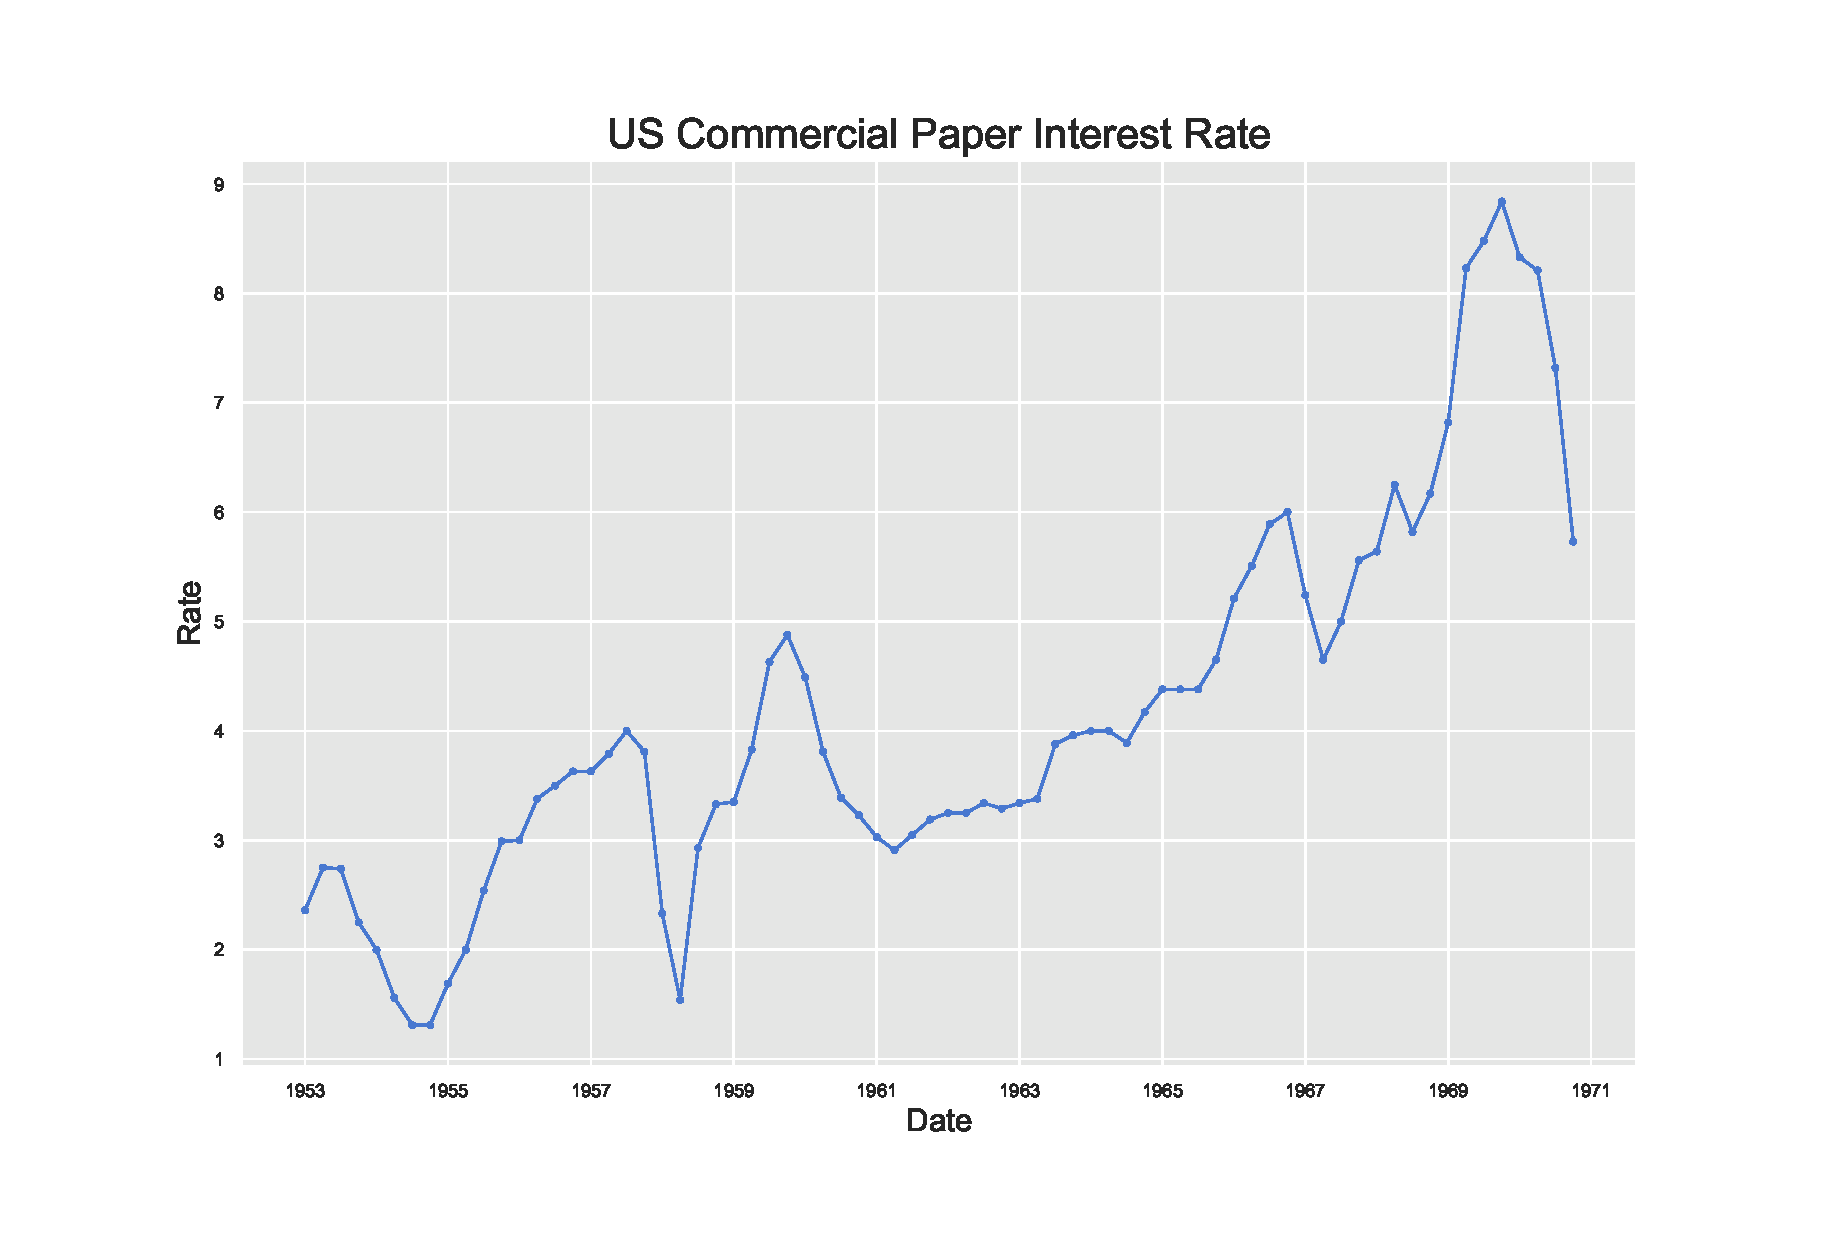
\includegraphics[width=\textwidth]{chapters/chapter_uvts/figures/uscompaper.eps}
	\caption{U.S. Commercial Paper Interest Rate. \label{fig:exchratefirst}}
	\end{figure}
The use of the unit root test statistics will become apparent when we discuss pairs trading based on co-integration (see Chapter~\ref{ch:stat_ts}). A precondition for forming co-integrated pairs is that each series must be non-stationary on its own. \xqed
\end{ex}



% Forecasting for ARIMA Processes
\subsection{Forecasting for ARIMA Processes}


Given a realization of ARIMA($p,d,q$) process through time t, $\{ Y_s, s \leq t \}$, we consider the problem of forecasting of future values $Y_{t+l}, l = 1,2, \ldots$. For this purpose, it is assumed that the model for $\{ Y_t \}$ is known exactly including the values of the model parameters. Although, in practice, the model parameters are estimated from available sample data, errors due to estimation of parameters will not have too much effect on forecast properties for sufficiently large sample sizes. Also, the practical problem of future values based on the finite past sample data $Y_1, \ldots, Y_T$ will be considered briefly, but results based on the infinite past data assumption usually provide an adequate approximation to the finite past data prediction problem. \\


\noindent \textbf{Minimum Mean Squared Error Prediction} \\


Before presenting details of forecasting for ARIMA processes, we review some basic principles concerning prediction in a more general context. Let $Y$ be a r.v. and let $X = (X_1, \ldots, X_p)'$ be an $p$-dimensional random vector related to $Y$, and consider the problem of predicting (estimating) the unknown value of $Y$ by some function of $X$, say $\hat{Y} = g(x)$. The mean squared error (MSE) of a predictor $\hat{Y}$ is $E[(Y - \hat{Y})^2]$. We refer to the minimum mean squared error (minimum MSE) predictor of $Y$ as that function $\hat{Y} = g^*(X)$ such that, among all possible functions of $X$, $\hat{Y}$ minimizes the MSE $E[(Y - \hat{Y})^2]$. Then it is well-known that the \emph{minimum mean squared error} predictor is given by $\hat{Y} = E(Y\;|\;X)$, the conditional expectation of $Y$ given $X$, with prediction error $e = Y - \hat{Y} = Y - E(Y\;|\;X)$. One can also restrict prediction to consider only linear functions of $X$, and hence consider the minimum MSE \emph{linear} predictor as the linear function $\hat{Y}^* = a + b' X$ which minimizes the prediction MSE among all linear functions of $X$. It is well-known that the minimum MSE linear predictor is
	\begin{equation} \label{eqn:2yhatstar}
	\hat{Y}^* = \mu_y + \Sigma_{yx}\,\Sigma_{xx}^{-1}(X - \mu_x)
	\end{equation}
with the prediction error $e^* = Y - \hat{Y}^*$ having mean zero and prediction MSE (variance)
	\begin{equation} \label{eqn:2varestar}
	\var(e^*) = \var(Y - \hat{Y}^*) = \sigma_y^2 - \Sigma_{yx}\,\Sigma_{xx}^{-1}\,\Sigma_{xy},
	\end{equation}
where $\mu_y = E(Y), \mu_x = E(X)$, $\sigma_y^2 = \var(Y)$, $\Sigma_{yx} = \cov(Y,X)$, and $\Sigma_{xx} = \cov(X)$. Note $\Sigma_{yx}$ is a $1 \times p$ row vector and $\Sigma_{xx}$ is a $p \times p$ variance-covariance matrix. Moreover, if the prediction error $e^* = Y - \hat{Y}^*$ of the best linear predictor is such that $E(e^*\;|\;X) = 0$ (e.g., if $e^*$ is independent of $X$), then $\hat{Y}^*$ is also the minimum MSE predictor, i.e. $\hat{Y}^* = \hat{Y} = E(Y\;|\;X)$ is a linear function of $X$ and the prediction error $e = e^* = Y - \hat{Y}$ has variance $\var(e^*)$ as given above in \eqref{eqn:2varestar}. \\


\noindent\textbf{Forecasting for ARIMA Processes and Properties of Forecast Errors} \\


For forecasting in the time series setting, we assume that the process $\{ Y_t \}$ follows an ARIMA$(p,d,q)$ model, $\phi(B)(1 - B)^d\,  Y_t = \theta(B) \varepsilon_t$, and we assume the white noise series $\varepsilon_t$ are mutually independent random variables. We are interested in forecasting the future value $Y_{t+l}$ based on observations $Y_t,Y_{t-1},\cdots$. From the result in previous section, the minimum MSE forecast of $Y_{t+l}$ based on $Y_t, Y_{t-1}, \ldots$, which we will denote as $\hat{Y}_t(l)$, is such that $\hat{Y}_t(l) = E(Y_{t+l} \;|\; Y_t,Y_{t-1},\ldots)$. The prediction $\hat{Y}_t(l)$ is called the lead $l$ or $l$-step ahead forecast of $Y_{t+l}$, $l$ is the lead time, and $t$ is the forecast origin.


To obtain a representation for $\hat{Y}_t(l)$, recall the ARIMA process has the ``infinite'' MA form $Y_t = \psi(B) \varepsilon_t = \sum_{i=0}^{\infty}\psi_i \varepsilon_{t-i},$ and hence a future value $Y_{t+l}$ at time $t+l$, relative to the current time or ``forecast origin'' t, can be expressed as
	\begin{equation} \label{eqn:2ytl}
	Y_{t+l} = \sum_{i=0}^\infty \psi_i \varepsilon_{t+l-i} = \sum_{i=0}^{l-1} \psi_i \varepsilon_{t+l-i} + \sum_{i=l}^\infty \psi_i \varepsilon_{t+l-i}.
	\end{equation}
The information contained in the past history of the $Y_t's, \{ Y_s, s \leq t \}$, is the same as that contained in the past random shocks $\varepsilon_t$'s (because the $Y_t$'s are generated by the $\varepsilon_t$'s). Also, $\varepsilon_{t+h}$, for $h > 0$ is independent of present and past values $Y_{t}, Y_{t-1}, \ldots$, so that $E(\varepsilon_{t+h} \;|\; Y_t,Y_{t-1},\ldots) = 0, h>0$. Thus
	\begin{equation} \label{eqn:2yhatt}
	\hat{Y}_t(l) = E(Y_{t+l} \;|\; Y_t,Y_{t-1},\ldots) = E(Y_{t+l} \;|\; \varepsilon_t, \varepsilon_{t-1}, \ldots) = \sum_{i=l}^\infty \psi_i \varepsilon_{t+l-i},
	\end{equation}
using the additional property that $E(\varepsilon_{t+l-i} \;|\; \varepsilon_t,  \varepsilon_{t-1}, \ldots) = \varepsilon_{t+l-i}$ if $i \geq l$. The $l$-step ahead prediction error is given by $e_t(l) = Y_{t+l} - \hat{Y}_t(l) = \sum_{i=0}^{l-1} \psi_i \varepsilon_{t+l-i}$. So we have $E[e_t(l)]=0$ and the mean squared error or variance of the $l$-step prediction error is
	\begin{equation} \label{eqn:2sigmasq}
	\sigma^2(l) = \var(e_t(l)) = E[e_t^2(l)] = \var \left(\sum_{i=0}^{l-1} \psi_i \varepsilon_{t+l-i} \right) = \sigma^2 \sum_{i=0}^{l-1} \psi_i^2,
	\end{equation}
with St.Dev. $(e_t(l)) = \sigma(l) = \sigma(1 + \psi_1^2 + \cdots + \psi_{l-1}^2)^{1/2}$. Note, in particular, that for $l = 1$ step we have $e_t(1) = Y_{t+1} - \hat{Y}(1) = \varepsilon_{t+1}$ with error variance $\sigma^2 = \var(\varepsilon_{t+1})$, so that the white noise series $\varepsilon_t$ can also be interpreted as the one-step ahead forecast errors for the process. Under the normality assumption that the $\varepsilon_t$ are normally distributed as i.i.d. $N(0, \sigma^2)$, the $l$-step ahead forecast errors $e_t(l) = Y_{t+l} - \hat{Y}_t(l) = \sum_{i=0}^{l-1} \psi_i \varepsilon_{t+l-i}$ will also be normally distributed with mean 0 and variance $\sigma^2(l) = \sigma^2 \sum_{i=0}^{l-1} \psi_i^2$. Hence, the conditional distribution of $Y_{t+l}$, given $Y_t,Y_{t-1}, \ldots$, is normal with mean $\hat{Y}_t(l)$ and variance $\sigma^2(l)$.


For forecasting purposes, the variance $\sigma^2(l)$ of the $l$-step forecast error provides a measure of the degree of accuracy of the point forecast $\hat{Y}_t(l)$. Along with the point forecast $\hat{Y}_t(l)$, we need to provide prediction intervals for the future observations $Y_{t+l}$ so that the degree of uncertainty of the point forecasts is properly reflected. From the preceding paragraph, it follows that the standardized variable $Z_t(l) = e_t(l) / \sigma(l)= ( Y_{t+l} - \hat{Y}_t(l) ) / \sigma(l)$ is distributed as standard normal $N(0,1)$, which is also the conditional distribution of this variable, given $Y_t, Y_{t-1}, \ldots$. Then, for example, from $0.90 = R[-1.65 < Z_t(l) < 1.65] = P[\hat{Y}_t(l) - 1.65\,\sigma(l) < Y_{t+l} < \hat{Y}_t(l) + 1.65\,\sigma(l)]$, it follows that a $90\%$ prediction interval (interval forecast) for $Y_{t+l}$ is given by $\hat{Y}_t(l) \pm 1.65 \sigma(l)$, where $\sigma(l) = \sigma( \sum_{i=0}^{l-1} \Psi_i^2 )^{1/2}$. Prediction intervals for other desired levels of confidence, $100(1 - \alpha)\%$, can be constructed similarly. Of course, in practice, estimates of $\sigma^2$ and of the weights $\psi_i$ based on the estimates $\hat{\phi}_i$ and $\hat{\theta}_i$ of parameters in the ARIMA model obtained from the sample data will actually be used in estimating the standard deviation $\sigma(l)$ of the forecast errors and in forming the prediction intervals. \\


\noindent\textbf{Eventual Forecast Function for ARIMA Processes} \\


It can be shown that the forecast function $\hat{Y}_t(l)$, considered as a function of the lead time $l$ with the origin `$t$' fixed, satisfies the linear difference equation
	\begin{equation} \label{eqn:2twoyhat}
	\hat{Y}_t(l) = \sum_{i=1}^{p+d}  \phi_i \hat{Y}_t(l-i) + \delta \quad \text{for } l > q.
	\end{equation}
We can express this relation as $\phi^*(B)\, \hat{Y}_t(l) = \delta$, for $l > q$, where the backshift operator $B$ operates on the lead time $l$, with origin $t$ fixed. Hence for $l > q - p - d$, the function $\hat{Y}_t(l)$, which will be referred to as the \emph{eventual forecast function}, has the features of solution to the difference equation of order $p + d$. So, in general, as a function of $l$, $\hat{Y}_t(l)$ can consist of a mixture of polynomial terms, exponential decaying terms, and damped (and undamped) sinusoidal terms. The exact form of $\hat{Y}_t(l)$ is determined by the roots of the polynomial associated with the generalized AR operator $\phi^*(B) = \phi(B)(1 - B)^d$. 


\begin{ex}[IMA(1,1) Model]
 Let $Y_t - Y_{t-1} = \delta + \varepsilon_t - \theta\varepsilon_{t-1}$. Then, from \eqref{eqn:2ytl}--\eqref{eqn:2yhatt}, the forecasts are $\hat{Y}_t(1) = Y_t + \delta -\theta\varepsilon_t$, $\hat{Y}_t(2) = Y_t(1) + \delta = Y_t -\theta\varepsilon_t + 2\delta$, and in general,
	\[
	\hat{Y}_t(l) = \hat{Y}_t(l-1) + \delta = Y_t - \theta\varepsilon_t + \delta(l) = \hat{Y}_t(1) + \delta(l-1),\quad l= 1, 2, \ldots
	\]
So the ``eventual'' forecast function $\hat{Y}_t(l)$ is a straight line with a deterministic (fixed) slope $\delta$, and an ``adaptive'' intercept $\hat{Y}_t(1) - \delta = Y_t - \theta \varepsilon_t$ which is random and is adaptive to the process values which occur through time t. The variance of the $l$-step ahead forecast error $e_t(l)$ is $\sigma^2(l) = \sigma^2 (1 + (l-1)(1-\theta)^2), l \geq1$. Hence, we see that the values $\sigma^2(l)$ increase without bound as the lead time $l$ increases, which is a general feature for (nonstationary) ARIMA processes with $d > 0$. Also notice from the infinite AR form of the model (with $\delta = 0$) with AR coefficients $\pi_i = (1-\theta\,)\theta^{i-1}$, $i \geq 1$, $Y_{t+1} = (1-\theta)\sum_{i=1}^\infty \theta^{i-1}Y_{t+1-i} + \varepsilon_{t+1}$, we have the representation $\hat{Y}_t(1) = (1-\theta)\sum_{i=1}^\infty \theta^{i-1} Y_{t+1-i}$. This provides the exponential smoothing, or exponentially weighted moving average (EWMA), form of the one-step forecast $\hat{Y}_t(1)$ in the IMA(1,1). This model with a short term drift `$\delta$' is of immense interest in modeling the stock prices. \xqed
\end{ex}



% Stylized Models for Asset Returns
\section{Stylized Models for Asset Returns}


It is generally known that the equity market is extremely efficient in quickly absorbing information about stocks: When new information arrives, it gets incorporated in the price without delay. Thus the efficient market hypothesis, is widely accepted by financial economists. It is implied that neither technical analysts that study the past prices in an attempt to predict future prices nor fundamental analysts of financial information related to company earnings and asset values would carry any advantage over the returns obtained from a randomly selected portfolio of individual stocks.


The efficient market hypothesis is usually associated with the idea of the ``random walk'', which implies that all future price changes represent random departures from past prices. As stated in Malkiel (2012)~\cite{malkiel}: ``The logic of the random walk is that if the flow of information is unimpeded and information is immediately reflected in stock prices, then tomorrow's price change will reflect only tomorrow's news and will be independent of the price changes today. But news by definition is unpredictable, and, thus resulting price changes must be unpredictable and random.''


The random walk (RW) model (Example~\ref{ex:driftwalk}) without the drift term can be stated as:
	\begin{equation} \label{eqn:2pteq}
	p_t = p_{t-1} + \varepsilon_t,
	\end{equation}
where $\varepsilon_t \sim N(0,\sigma^2)$ i.i.d and $p_t = \ln{(P_t)}$. Note as observed earlier, this model is a particular case of AR(1) model if the constant term is assumed to be zero and the slope, $\phi$, is assumed to be one. Thus, the RW model is a non-stationary model and considering $\varepsilon_t = p_t - p_{t-1}=r_t$ is the differencing of the series, $p_t$, makes the series $\varepsilon_t$ stationary. Note $r_t \approx \frac{P_t - P_{t-1}}{P_{t-1}}$,  the returns are purely random and are unpredictable. For any chronological data the decision concerning the need for differencing is based, informally, on the features of time series plot of $p_t$, its sample autocorrelation function; that is, its failure to dampen out sufficiently quickly. \\


\noindent\textbf{Testing for a RW model:} Consider the AR(1) model $p_t = \phi p_{t-1} + \varepsilon_t$, $t = 1,\ldots,T$ and $p_0$ is fixed; we want to test $\phi = 1$. The details of this test are given in Section~\ref{sec:diffornot}, along with the table of the percentiles of the distribution of the test statistics. While the results for testing for non-stationarity for higher order autoregressive models were discussed earlier, the price series once differenced does not generally exhibit autocorrelation structure that requires modeling beyond AR(1).


It will become obvious in subsequent discussions, that in order to exploit any pattern in the returns, one has to look beyond linear time dependencies. We observe a series of established stylized facts regarding price (return). \\


\noindent\textbf{Stylized fact 1: Absence of Autocorrelation in returns:} Linear autocorrelations are often insignificant for a lower frequency data. 


To illustrate the main ideas, we consider the exchange rate between USD and GBP; these are daily closing rates from January 4, 1999 to September 16, 2013. The time series plot of the data in (Figure~\ref{fig:exchrate}) clearly indicates that the price is non-stationary and it is confirmed by the never dying autocorrelation function in (Figure~\ref{fig:exchrate}). The LS estimates $\hat{\phi}= 0.9996$, $s_e= 0.00958$ and $\sum_{t=2}^T p_{t-1}^2 = 10431$, provides a value of $\hat{\tau} = -0.001$ from \eqref{eqn:hattaunew} which confirms that the series is a random walk. The differenced series, $r_t = \ln{(p_t)} - \ln{(p_{t-1})}$ is plotted in (Figure~\ref{fig:exchrate}) and its autocorrelation function is given in (Figure~\ref{fig:exchrate}). Thus it would appear that return series is a white noise process.


Many industry analysts tend to look at not just the closing price but also the so called price bars that consist of open, high, low and close prices in discrete time intervals. Select averages over these four quantities are monitored to study the stock momentum. Two such quantities discussed in the literature are pivot, the average of high, low and close prices; and mid-range, the average of high and low prices. The plot of the pivot for the exchange rate is overlaid on the closing price in Figure~\ref{fig:timegbp}. It is not easy to distinguish between the two series from this plot, but an important property of the (aggregated) pivot series is worth-noting here. The autocorrelation of the returns dated on pivot series at lag 1 is quite significant (Figure~\ref{fig:timegbp}). This happens mainly due to `aggregation' of data as observed by Working (1960)~\cite{working1960note} and by Daniels (1966)~\cite{daniels1966autocorrelation}. Working (1960)~\cite{working1960note} shows that if the average is computed over `$m$' terms in each time segment (in this illustration, a day) the first order correlation is $\frac{(m^2-1)}{2(2m^2+1)}$. When $m= 3$, we can expect the lag 1 autocorrelation to be about 0.21. Daniels (1966)~\cite{daniels1966autocorrelation} observes that we could expect lag 1 autocorrelation in the order of 0.4 for the mid-range series. Thus, the main point of this discussion is that the aggregation of prices (which is the basis of several low-frequency analysis) induces the autocorrelation by construction, but it does not mean that there is market inefficiency.
	\begin{figure}[!ht]
	\centering
	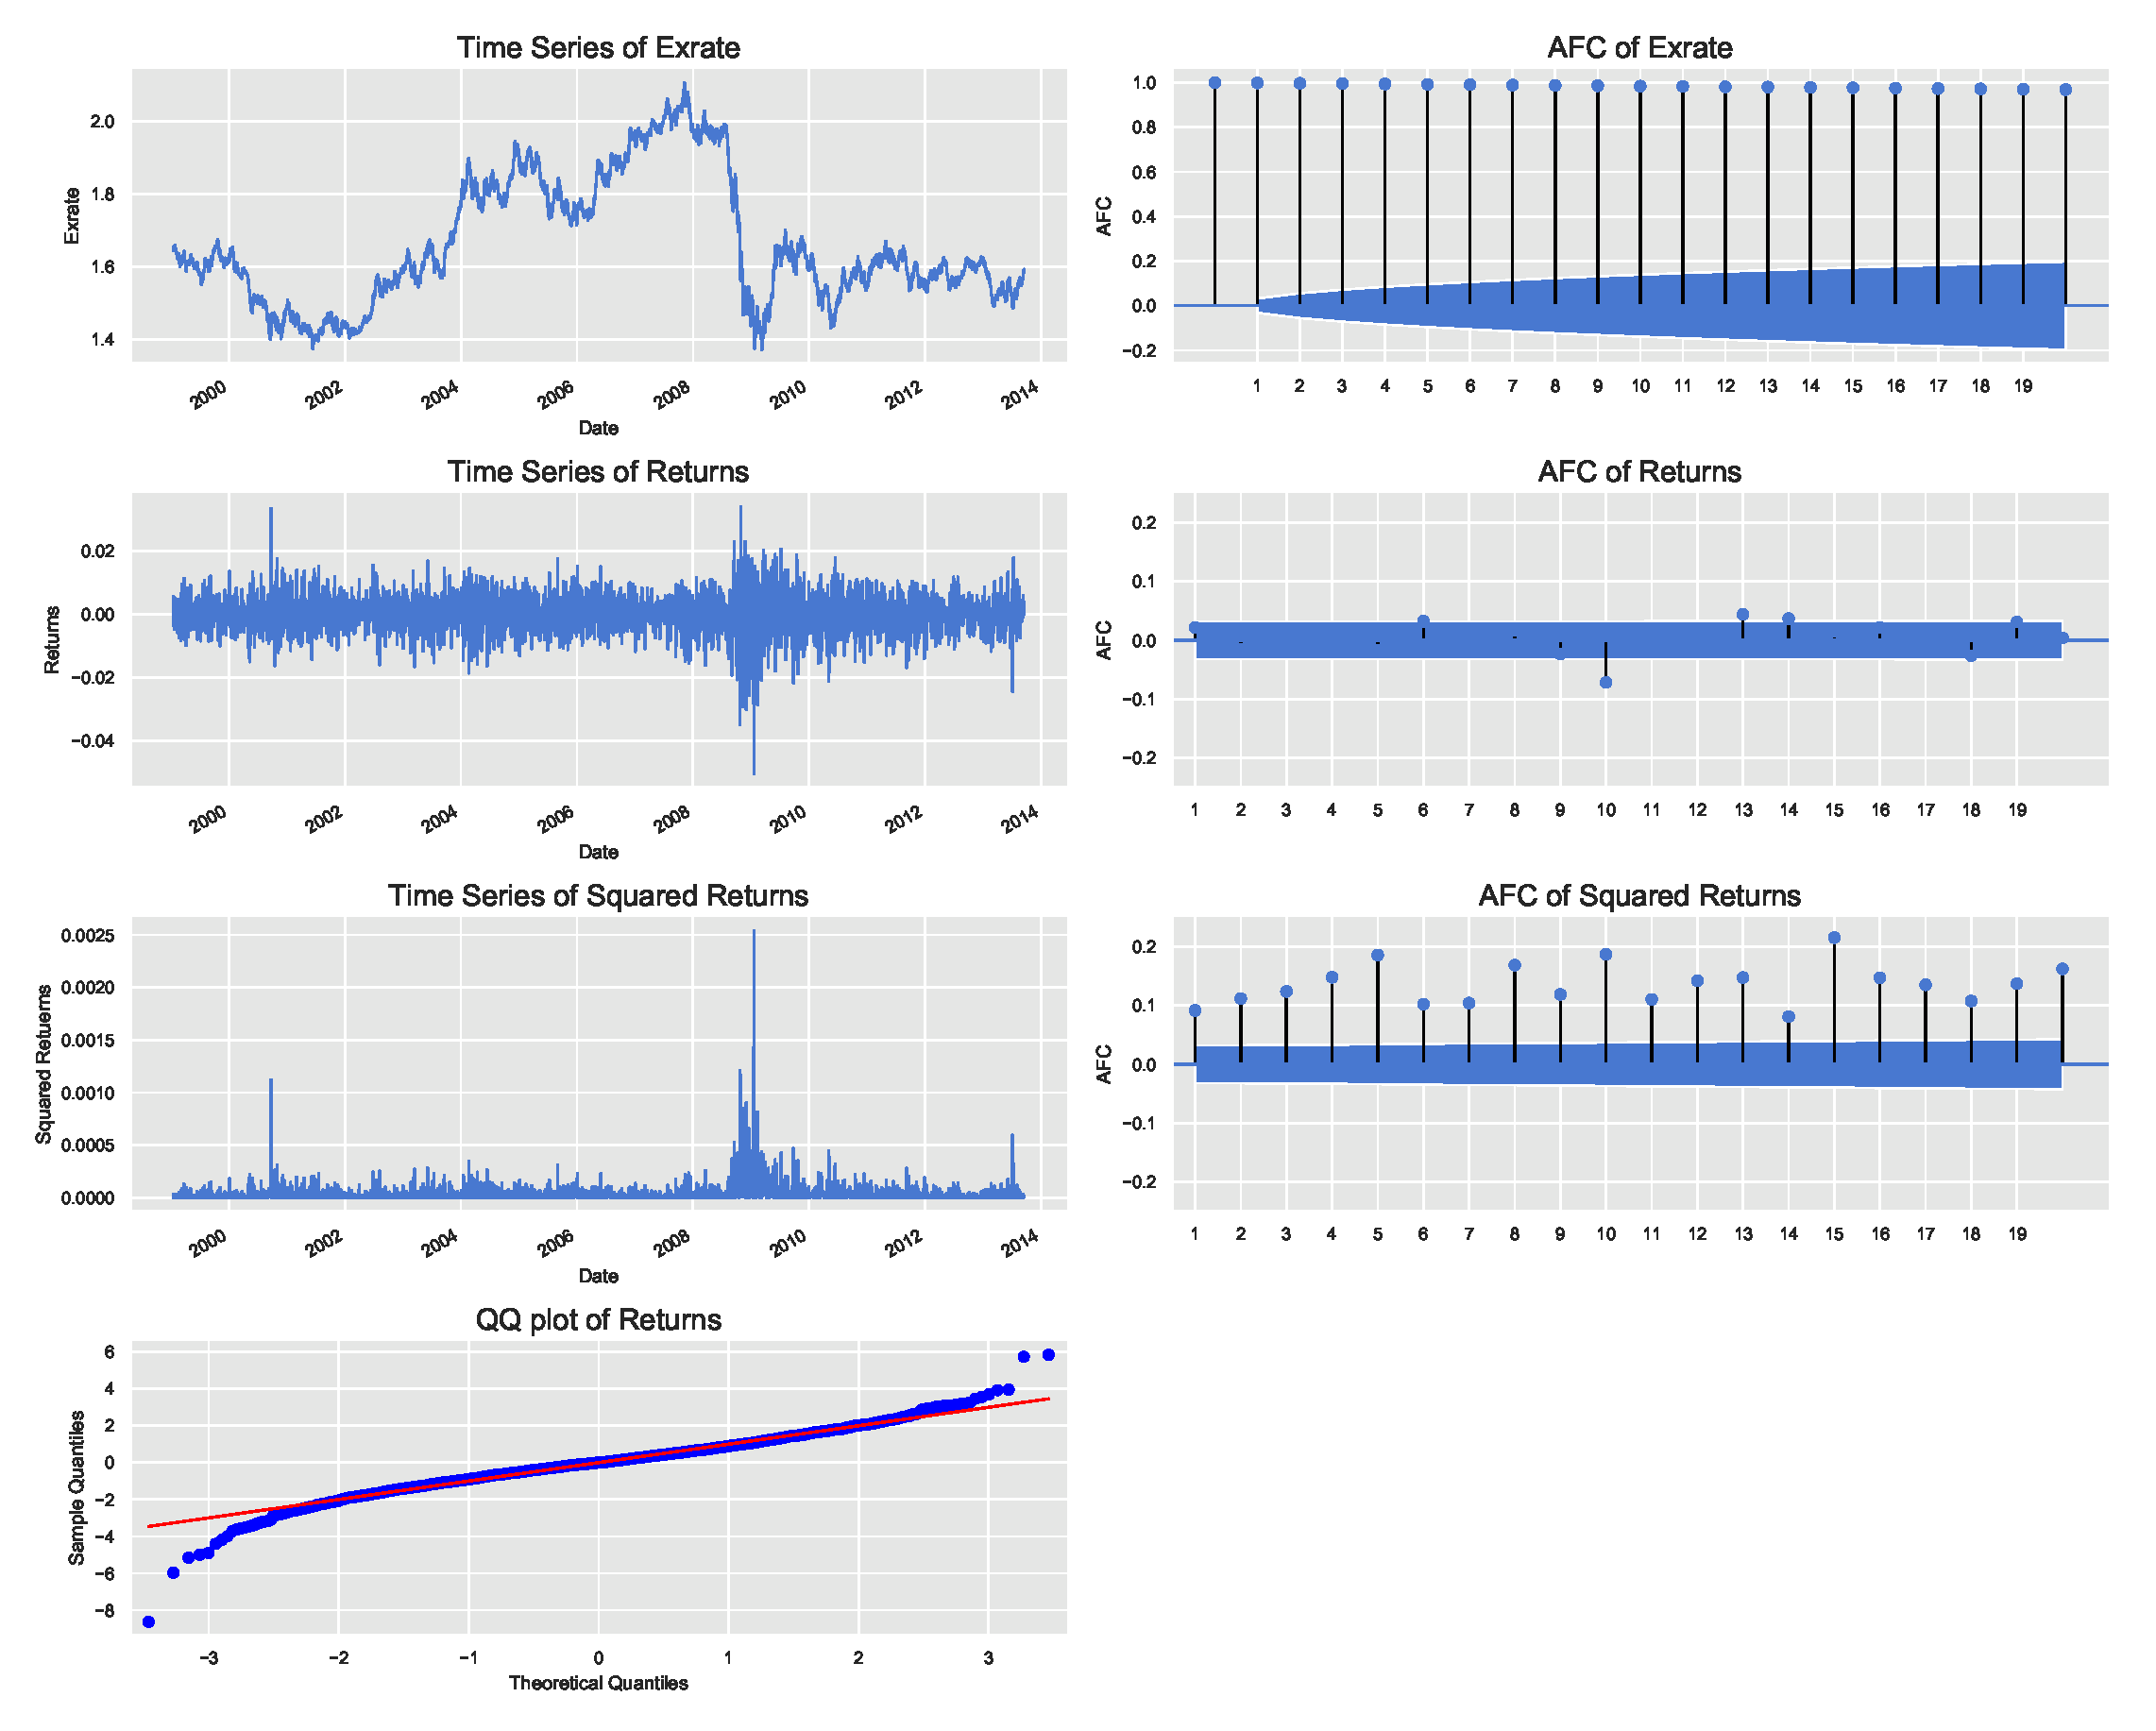
\includegraphics[width=\textwidth]{chapters/chapter_uvts/figures/31graphs.eps}
	\caption{Exchange rate related plots. \label{fig:exchrate}}
	\end{figure}

	\begin{figure}[!ht]
	\centering
	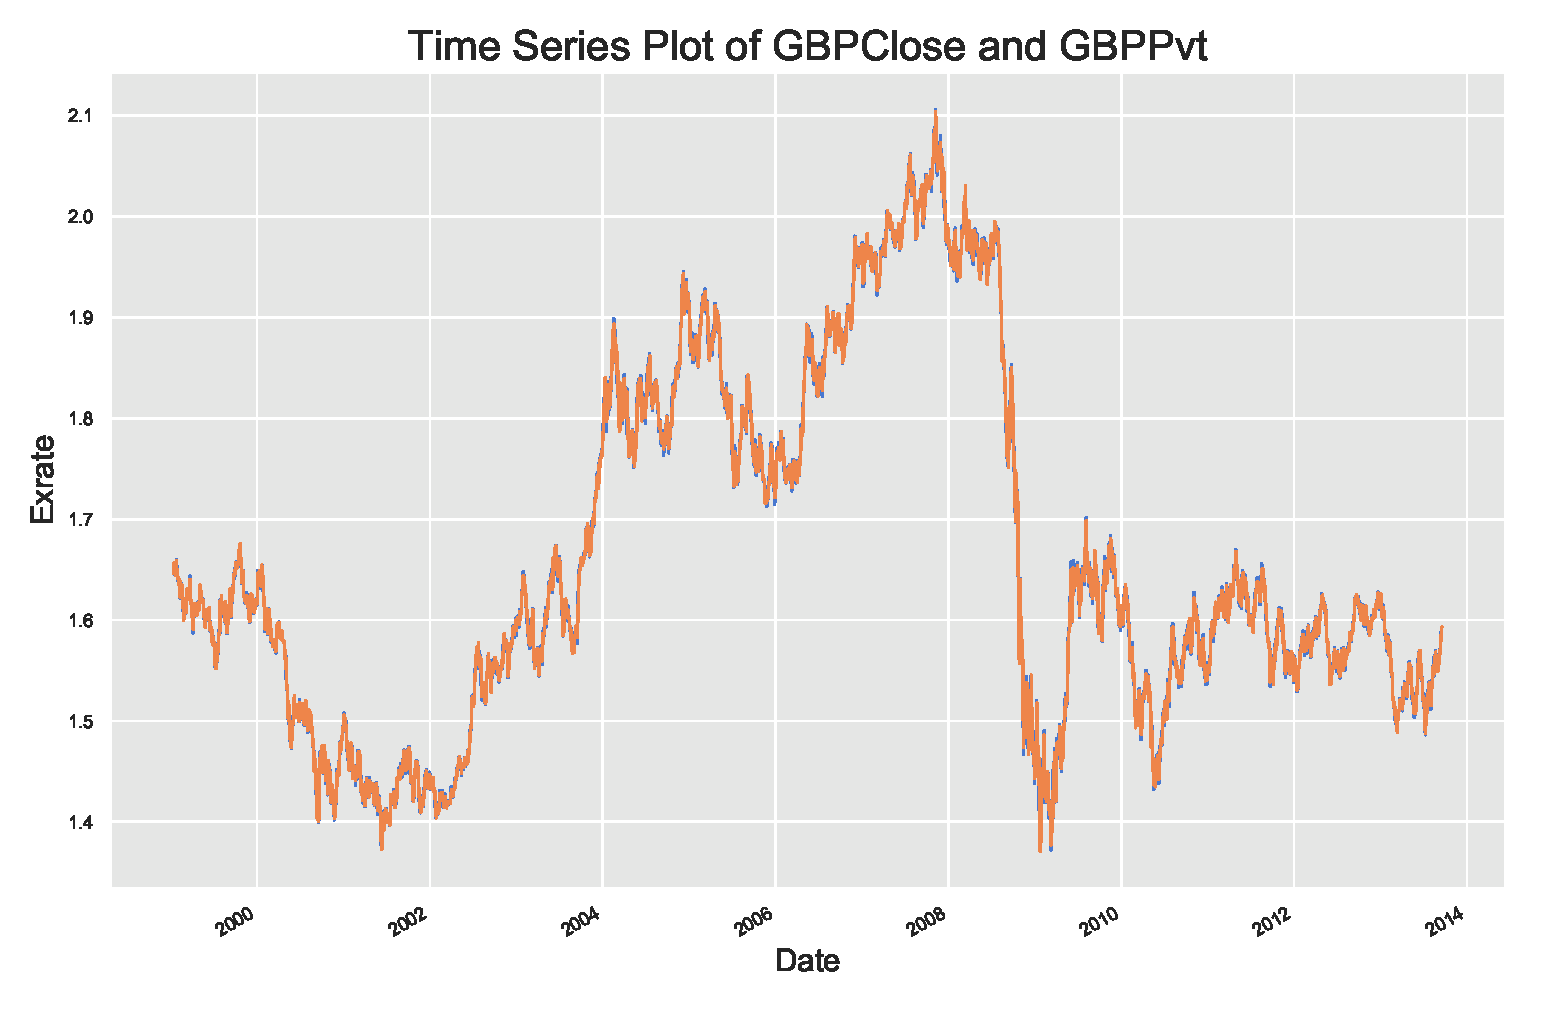
\includegraphics[width=\textwidth]{chapters/chapter_uvts/figures/Sec2-4Fig4.eps}
	\caption{Times series plot of GBPClose, GBPPvt. \label{fig:timegbp}}
	\end{figure}
	
	\begin{figure}[!ht]
	\centering
	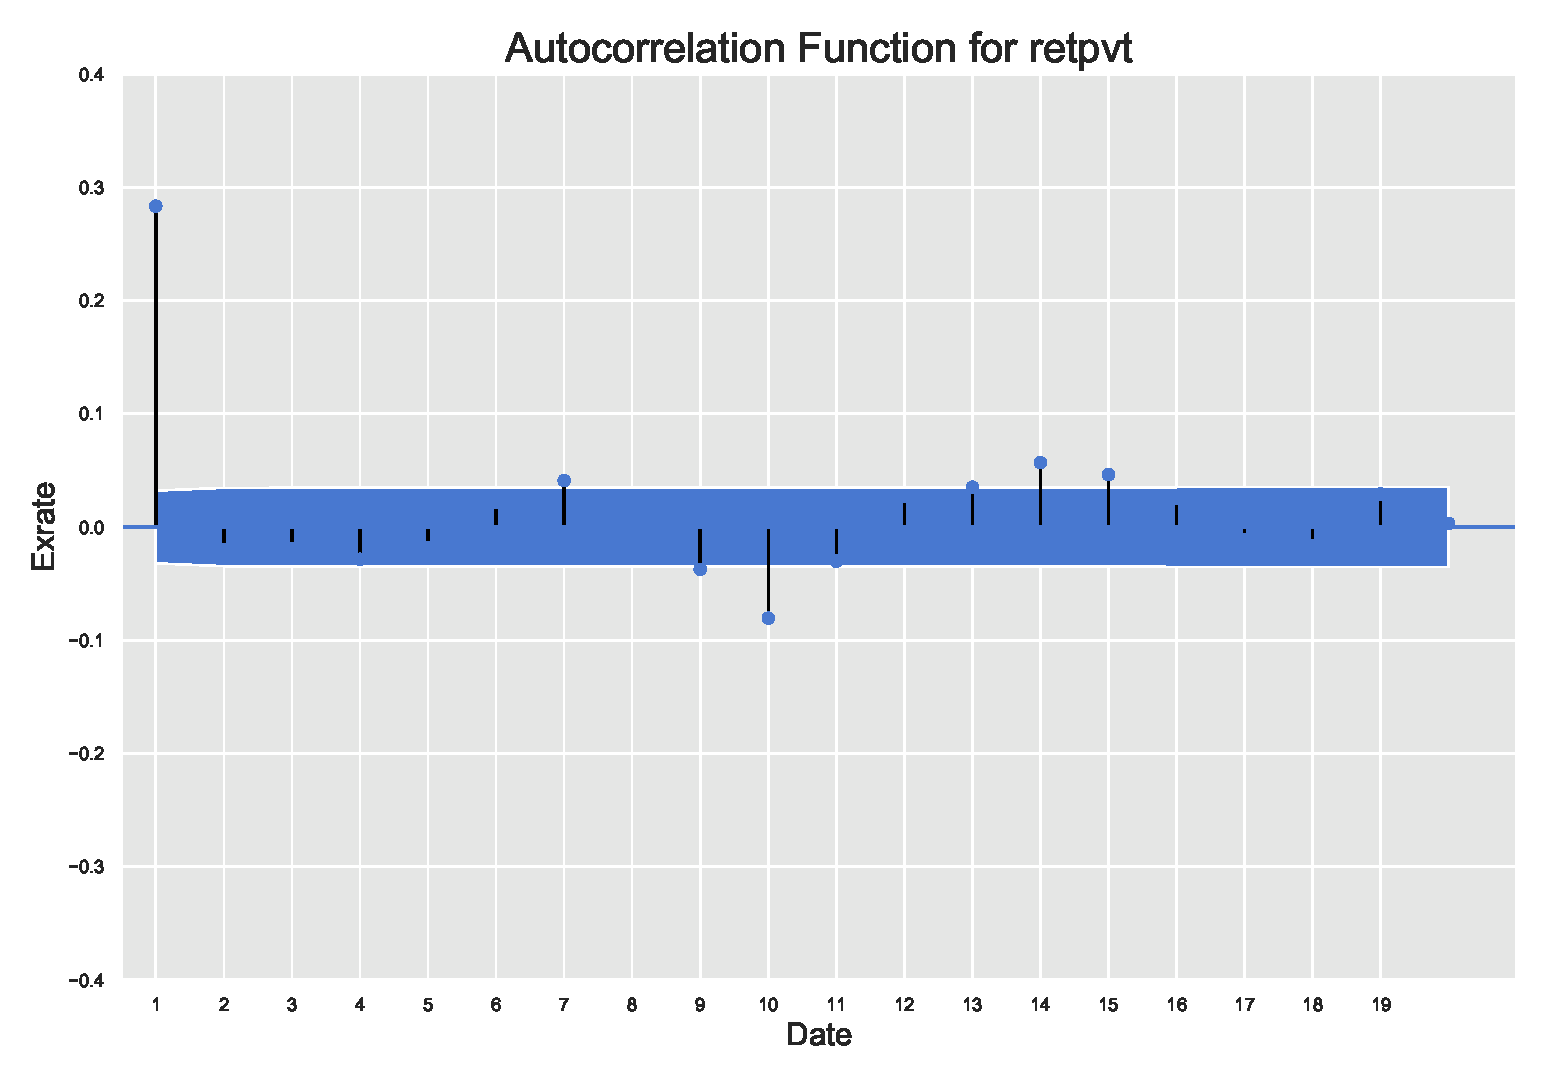
\includegraphics[width=\textwidth]{chapters/chapter_uvts/figures/Sec2-4Fig5.eps}
	\caption{Autocorrelation function for rtpvt. \label{fig:autocorrtpvt}}
	\end{figure}
An assumption of the random walk model that is often made is that the errors (returns)
follow a normal distribution. But in practice, the errors (or returns) tend to have heavier tails than the normal. We suggest using the quantile-quantile plot which is quite sensitive to even modest deviations from normality and also a test based on the properties of normal distribution. An omnibus test based on the skewness ($=0$ for normal) and the kurtosis ($=3$ for normal) is Jarque-Bera test:
	\begin{equation} \label{eqn:2JB}
	\text{JB }= n \left( \frac{\widehat{\text{SK}}^2}{6} + \frac{(\hat{K} - 3)^2}{24} \right) \sim \chi_2^2,
	\end{equation}
where $\text{SK} \text{(ewness)}= E( \frac{X-\mu}{\sigma} )^3, \text{K} \text{(urtosis)} = E( \frac{X-\mu}{\sigma} )^4$. The corresponding sample numbers are substituted in JB (see Jarque and Bera (1980)~\cite{jarque80}). Alternatively, the probability (Q--Q) plot of $r_t = \ln{(p_t)} - \ln{(p_{t-1})}$ as given in Figure~\ref{fig:exchrate} clearly indicates that the distribution has somewhat heavy tails. (For this data $\widehat{SK} = -0.31$ and $\hat{K} = 3.67$ resulting in $\text{JB}= 129.7$ with $n= 3236$, thus rejecting the normal distribution.) \\


\noindent\textbf{Stylized fact 2:} Heavy Tails: The returns are likely to display a heavy
tailed distribution such as a power-law or Pareto. \\


\noindent\textbf{Stylized fact 3:} Asymmetry: When prices fall, they tend to fall faster
than when they tend to rise, thus drawdowns tend to be larger than upward rises. \\


These stylized facts are particularly important for risk management of strategies, and how they could be incorporated in trading decisions is still a subject of much research and will be discussed later. The thicker tail distribution warrants that the chance of extreme values are more likely to occur than what is predicted by a normal distribution and the asymmetry indicates that there is a difference between positive and negative sides of variance (volatility). 



% Time Series Models for Aggregated Data
\section{Time Series Models for Aggregated Data: Modeling the Variance}


In the ARMA$(p,q)$ model $\phi(B)Y_t= \delta + \theta(B) \,\varepsilon_t$ for series $\{ Y_t \}$, when the errors $\varepsilon_t$ are \emph{independent} r.v.'s (with the usual assumptions of zero mean and constant variance $\sigma^2$), an implication is that the \textit{conditional} variance of $\varepsilon_t$ given the past information is a constant not depending on the past. This, in turn, implies the same feature for $l$-step ahead forecast errors $e_t(l) = \sum_{i=0}^{l-1} \psi_i \varepsilon_{t+l-i}$. However, in some settings, particularly for financial data, the variability of errors may exhibit dependence on the past variability. Modeling the variance, which is essential for studying the risk-return relationship is an important topic in finance. \\


\noindent \textbf{Autoregressive Conditional Heteroscedastic (ARCH) Models} \\


The autoregressive conditional heteroscedastic (ARCH) models were originally proposed by Engle (1982)~\cite{engle1982}, Engle and Kraft (1983)~\cite{engle1983}, to allow for the conditional error variance in an ARMA process to depend on the past squared innovations, rather than be a constant as in ARMA models with independent errors. For example, an AR$(p)$ process with ARCH$(q)$ model errors is given as $Y_t = \sum_{i=1}^p\phi_iY_{t-i} + \delta + \varepsilon_t$, where, $E(\varepsilon_t \;|\; \varepsilon_{t-1},\varepsilon_{t-2},\ldots)= 0$ and
	\begin{equation} \label{eqn:2ht}
	h_t= \var(\varepsilon_t \;|\; \varepsilon_{t-1}, \varepsilon_{t-2}, \ldots) = \omega_0 + \sum_{i=1}^q \omega_i \varepsilon_{t-i}^2
	\end{equation}
with $\omega_0 > 0$ and $\omega_i \geq 0$ for $i= 1, \ldots, q$. In the generalized ARCH (GARCH) model, introduced by Bollerslev (1986)~\cite{bollerslev1986}, it is assumed that
	\begin{equation} \label{eqn:2secondht}
	h_t = \omega_0 + \sum_{i=1}^q \omega_i \varepsilon_{t-i}^2 + \sum_{i=1}^k \beta_i h_{t-i},
	\end{equation}
where $\beta_i \geq 0$ for all $i = 1,\ldots,k$. Much subsequent research on and applications of the ARCH and GARCH models have occurred since the publication of their research papers.


Let us briefly discuss some basic results and implications of the ARCH and GARCH models. The errors $\varepsilon_t$ in the model have zero mean, since $E(\varepsilon_t) = E[E(\varepsilon_t \;|\; \varepsilon_{t-1} \ldots)] = 0$, and they are serially uncorrelated; that is, $E(\varepsilon_t \varepsilon_{t-j}) = 0$ for $j \not= 0$ (since for $j > 0$, for example, $E(\varepsilon_t \varepsilon_{t-j}) = E[E(\varepsilon_t \varepsilon_{t-j} \;|\; \varepsilon_{t-1} \ldots)] = E[\varepsilon_{t-j} E(\varepsilon_t \;|\; \varepsilon_{t-1} \ldots)] = 0$). But the $\varepsilon_t$ are not mutually independent r.v.'s since they are inter-related through their conditional variances (i.e., their second moment). We will also assume that the $\varepsilon_t$ have equal unconditional variances, $\var(\varepsilon_t) = \sigma^2$, for all $t$, so they are weakly stationary. Consider then, the simple case of the first-order ARCH or ARCH(1) model,
	\begin{equation} \label{eqn:2htE}
	h_t = \omega_0 + \omega_1 \varepsilon_{t-1}^2,
	\end{equation}
Assuming that $\omega_1 < 1$ ($\omega_0$ and $\omega_1 \geq 0$ is always assumed), the \emph{unconditional} variance of $\varepsilon_t$ is $\sigma^2= \var(\varepsilon_t) = \frac{\omega_0}{1 - \omega_1}$, since $\sigma^2 = E(\varepsilon_t^2) = E[E(\varepsilon_t^2 \,|\, \varepsilon_{t-1}, \ldots)] = E[\omega_0 + \omega_1\varepsilon_{t-1}^2] = \omega_0 + \omega_1\sigma^2$. Therefore, the conditional variance of $\varepsilon_t$ can be written as
	\begin{equation} \label{eqn:2htw}
	h_t = \omega_0 + \omega_1 \varepsilon_{t-1}^2 = \sigma^2 + \omega_1 (\varepsilon_{t-1}^2 - \sigma^2),
	\end{equation}
or in the form of deviation from the unconditional variance as $h_t - \sigma^2= \omega_1 (\varepsilon_{t-1}^2 - \sigma^2)$. So the conditional variance will be above the unconditional variance whenever $\varepsilon_{t-1}^2$ exceeds its unconditional variance $\sigma^2$. If $\varepsilon_t$ were conditionally normally distributed, given the past, the fourth unconditional moment $E(\varepsilon_t^4)$ will exceed $3 \sigma^4$ (the value in the normal distribution), so that the marginal distribution of $\varepsilon_t$ will exhibit fatter tails that the normal distribution. Conditional variances of multi-step ahead forecast errors can also be established to depend on the past squared errors. 


These basic results indicated that the properties of the ARCH(1) model also tend to hold for the higher order ARCH$(q)$ models. A basic impact of the ARCH errors in a process is in assessment of the accuracy of forecast, since the forecast errors will have conditional variances (given the past) that depend on the past. This allows for formation of correct and more informative (conditional) prediction intervals that would be obtained under the usual assumption that conditional error variances were constant independent of the past.


Now consider briefly the popular GARCH(1,1) model, $h_t = E(\varepsilon_t^2 \;|\; \varepsilon_{t-1}, \ldots) = \omega_0 + \omega_1\varepsilon_{t-1}^2 + \beta_1h_{t-1}$. Similar to the result for the ARCH(1) model, assuming that $\omega_1 + \beta_1 < 1$, it is readily shown that the unconditional variance of $\varepsilon_t$ is equal to $\sigma^2 = \var(\varepsilon_t) = \omega_0/[1 - (\omega_1 + \beta_1)]$. Let $v_t = \varepsilon_t^2 - h_t$, so that the random variables $v_t$ have zero mean, and they are serially uncorrelated since
	\[
	E( (\varepsilon_t^2 - h_t) (\varepsilon_{t-j}^2 - h_{t-j}) )= E[(\varepsilon_{t-j}^2 - h_{t-j}) E\{(\varepsilon_t^2 - h_t) \,|\, \varepsilon_{t-1},\ldots\}] = 0.
	\]
Then, since $h_t = \varepsilon_t^2 - v_t$, note that the GARCH(1,1) model can be rearranged as $\varepsilon_t^2 - v_t = \omega_0 + \omega_1\varepsilon_{t-1}^2 + \beta_1(\varepsilon_{t-1}^2 - v_{t-1})$, or
	\begin{equation} \label{eqn:2ept}
	\varepsilon_t^2 = \omega_0 + (\omega_1 + \beta_1)\varepsilon_{t-1}^2 + v_t - \beta_1v_{t-1}.
	\end{equation}
This form reveals that the process of squared errors, $\{\varepsilon_t^2\}$, follows an ARMA(1,1) model with uncorrelated innovations $v_t$ (however, the $v_t$ are conditionally heteroscedastic and more strongly are Martingale differences. Although this process looks like a linear process, it is not, since $ \{ v_t \}$ are uncorrelated but dependent. This fact motivates the use of the ACF and PACF of the squares $\varepsilon_t^2$ for model specification and for basic preliminary checking for the presence of ARCH/GARCH effects in the errors $\varepsilon_t$. In practice, a starting point would be examination of the sample ACF and PACF of the squared residuals $\hat{\varepsilon}_t^2$, where $\hat{\varepsilon}_t$ are residuals obtained from fitting of a usual ARMA$(p,q)$ model. The correspondence between ARCH and ARMA is further noted via the condition, $0 < \sum_{i=1}^q \omega_i < 1$, that implies the roots of its characteristic equation lie outside the unit circle (like a causal ARMA).


For maximum likelihood (ML) estimation of models with ARCH or GARCH errors, assuming that $\varepsilon_t$ is conditionally normally distributed as $N(0,h_t)$, we have the log-likelihood function (apart from some initial conditions) given by $\log(L) = -\frac{T}{2} \log(2\pi) - \frac{1}{2} \sum_{t=1}^T \log(h_t) - \frac{1}{2} \sum_{t=1}^T \varepsilon_t^2/h_t$. Maximum likelihood estimation procedures, properties of the estimators, and Lagrange multiplier (LM) and likelihood ratio (LR) procedures for testing for the presence of ARCH effects in the conditional variances of the $\varepsilon_t$ have been considered by Engle (1982)~\cite{engle1982} and Weiss (1984)~\cite{weiss1984}, among others.


As there are other excellent sources to learn about ARCH and GARCH models (see Tsay (2010)~\cite{tsay}, Chapter~\ref{ch:ch_uvts}), we have limited our discussion to some basic details. \\


\noindent\textbf{Preliminary Testing for ARCH Effect:} This is an omnibus test similar to Ljung-Box test that examines the presence of autocorrelation up to certain number of lags, which is equivalent to testing, $H_0: \alpha_1 = \alpha_2= \cdots = \alpha_q = 0$ in the model
	\begin{equation} \label{eqn:2eptsq}
	\varepsilon_t^2 = \alpha_0 + \alpha_1 \varepsilon_{t-1}^2 + \cdots + \alpha_q \varepsilon_{t-q}^2 + a_t,
	\end{equation}
where $a_t$ is white noise series; note that $\{ a_t \}$ does not need to follow a normal distribution. The usual $F$-test used in regression can be applied here; Let $R^2$ be the coefficient of determination that result from \eqref{eqn:2eptsq} when $\hat{\varepsilon}_t$'s are used; then
	\begin{equation} \label{eqn:2F}
	F = \frac{R^2/q}{(1 - R^2)/(T - 2q - 1)} \sim \chi^2/q.
	\end{equation}
We use $\chi^2$ instead of $F$ due to the fact that $\varepsilon_t$'s are estimated quantities. More informally, one could use the ACF of $\hat{\varepsilon}_t^2$ and if any of the autocorrelations are out of the normal bounds, $\pm 2/\sqrt{T}$, we may examine further for ARCH effects. \\


\noindent\textbf{GARCH vs ARCH:} While ARCH models care for the time dependence in volatilities and have elegant properties such as having excessive kurtosis (matching the empirical finding related to asset returns), they tend to overpredict the volatility and treat both negative and positive, $\varepsilon_t$'s symmetrically. To overcome some of these issues and as well as to come up with a more parsimonious representation (as in AR vs ARMA considerations) GARCH models stated in \eqref{eqn:2ept} are proposed. \\


\noindent\textbf{IGARCH:} The variance can persist for extended periods and can change at different time spans, thus leading to non-stationary behavior. In the GARCH(1,1) model, it is possible that $w_1 + \beta_1 = 1$, so that IGARCH(1,1) (Integrated GARCH) can be written as
	\begin{equation} \label{eqn:2eptsqrt}
	\varepsilon_t = \sqrt{h_t} \cdot a_t, \quad h_t = w_0 + w_1h_{t-1} + (1 - w_1) \varepsilon_{t-1}^2.
	\end{equation}
If $h_t$ is proxied by $\varepsilon_t^2$, the above model leads to $\varepsilon_t^2 - \varepsilon_{t-1}^2 = w_0 + w_1(\varepsilon_{t-1}^2 - \varepsilon_{t-2}^2)$, which is similar in form to non-stationary autoregressive model. In practice because of frequent level shifts in volatility, IGARCH appears to be a natural model to fit. Because the IGARCH(1,1) is similar to ARIMA(0,1,1), the model can be taken as an exponential smoothing model for the $\varepsilon_t^2$ series; By iterative substitutions, we can show that
	\begin{equation} \label{eqn:2ht1w}
	h_t = (1 - w_1) \big( \varepsilon_{t-1}^2 + w_1 \varepsilon_{t-2}^2 + w_1^2 \varepsilon_{t-3}^2 \cdots \big),
	\end{equation}
where $w_1$ can be taken as a discount factor. \\


\noindent\textbf{Prediction Performance of GARCH:} The predictive power of GARCH based on ex-post forecast evaluation criteria tend to suggest that the model provides poor forecasts, although the in-sample parameter estimates turn out to be highly significant. As Andersen and Bollerslev (1998)~\cite{andersen1998} note, in the model \eqref{eqn:2ept}, the latent volatility, $h_t$, evolves over time. The approach to evaluate the performance of the model for $h_t$ via $\hat{\varepsilon}_t^2$ is not appropriate. While $\hat{\varepsilon}_t^2$ provides an unbiased estimate of $h_t$, it is a noisy measurement due to idiosyncratic error terms associated with it; these error terms maybe due to the result of compounding frictions in the trading process. This will be further clarified when we discuss the analysis of high-frequency data. \\


\noindent \textbf{Time--Varying ARCH Processes (tvARCH):} The underlying assumptions of ARCH models is stationarity and with changing pace of economic conditions, the assumption of stationarity is not appropriate for modeling financial returns over long intervals. We may obtain a better fit by relaxing the assumption of stationarity. Dahlhaus and Subba Rao (2006)~\cite{dahlhaus2006} generalize the ARCH model with time-varying parameters:
	\begin{equation} \label{eqn:2eptsqrtht}
	\varepsilon_t = \sqrt{h_t}\cdot a_t, \quad h_t = w_0(t) + \sum_{j=1}^{\infty} w_j(t) \varepsilon_{t-j}^2,
	\end{equation}
which $a_t$'s are i.i.d. with mean zero and variance, one. By rescaling the parameters to unit intervals, the tvARCH process can be approximated by a stationary ARCH process. A broad class of models resulting from \eqref{eqn:2eptsqrtht} can be stated as:
	\begin{equation} \label{eqn:2eptN}
	\varepsilon_{t,N} = \sqrt{h_{t,N}} \cdot a_t, \quad h_{t,N} = w_0 \left( \frac{t}{N} \right) + \sum_{j=1}^pw_j \left (\frac{t}{N} \right) \varepsilon_{t-j,N}^2
	\end{equation}
for $t= 1, 2, \ldots, N$. This model captures the slow decay of the sample autocorrelations in squared returns that is commonly observed in financial data which is attributed to the long memory of the underlying process. But tvARCH$(p)$ is a non-stationary process that captures the property of long memory.


Fryzlewicz, Sapatinas and Subba Rao (2008)~\cite{fryzlewicz2008} propose a kernel normalized-least squares estimator which is easy to compute and is shown to have good performance properties. Rewriting \eqref{eqn:2eptN} as
	\begin{equation} \label{eqn:2eptNsq}
	\varepsilon_{t,N}^2 = w_0 \left(\frac{t}{N}\right) + \sum_{j=1}^p w_j \left(\frac{t}{N}\right)\varepsilon_{t-j,N}^2 + (a_t^2 - 1)h_{t,N}^2
	\end{equation}
in the autoregressive form, the least squares criterion with the weight function, $k(u_0,\chi_{k-1,N})$, where $\chi_{k-1,N}' = (1,\varepsilon_{k-1,N}^2, \ldots, \varepsilon_{k-p,N}^2)$ is
	\begin{equation} \label{eqn:2Lt0}
	L_{t_0,N}(\alpha) = \sum_{k=p+1}^N \frac{1}{b_N} \;w \left(\frac{t_0-k}{b_N} \right) \frac{\left(\varepsilon_{k\cdot N}^2 - \alpha_0 - \sum_{j=1}^p \alpha_j \varepsilon_{k-j \cdot N}^2 \right)^2}{k(u_0, \chi_{k-1\cdot N})^2}.
	\end{equation}
Minimizing \eqref{eqn:2Lt0} yields, $\hat{a}_{t_0,N} = R_{t_0,N}^{-1} r_{t_0,N}$, where
	\begin{center}
	\begin{flalign} \label{eqn:2Rt0}
	&& R_{t_0,N}&= \sum_{k=p+1}^N \frac{1}{b_N}\ ; w \left(\frac{t_0-k}{b_N} \right) \frac{\chi_{k-1\cdot N} \chi_{k-1\cdot N}'}{k(u_0, \chi_{k-1\cdot N})^2} && \notag \\
	\text{and} && \phantom{x} & \phantom{x} && \\
	&& r_{t_0,N} &= \sum_{k=p+1}^N \frac{1}{b_N}\; w \left(\frac{t_0-k}{b_N}\right)\frac{\varepsilon_{k\cdot N}^2  \chi_{k-1\cdot N}}{k(u_0,\chi_{k-1\cdot N})^2}. && \notag
	\end{flalign}
	\end{center}
The kernel $w$ is a function defined on $[-\frac{1}{2},\frac{1}{2}]$ which is of bounded variation. The choice of weight function suggested is as follows: it is motivated by the differing variances at various values of $k$. Estimate,
	\begin{center}
	\begin{flalign} \label{eqn:2skN}
	&& \hat{\mu}_{t_0,N}&= \sum_{k=1}^N\frac{1}{b_N} \; w\left(\frac{t_0 - k}{b_N}\right)\varepsilon_{k\cdot N}^2 && \notag \\
	\text{and} && \phantom{x} & \phantom{x} && \\
	&& s_{k-1\cdot N} &= \sum_{j=1}^p\varepsilon_{k-j\cdot N}^2 && \notag
	\end{flalign}
	\end{center}
and use $k_{t_0,N}(s_{k-1},N) = \hat{\mu}_{t_0,N} + s_{k-1\cdot N}$ as the weight function. Thus the estimation is a two-stage scheme. For the bandwidth selection, the cross-validation method based on a subsample of the observations is suggested.


The methodology presented here is useful because of the changing nature of financial volatility. Real data applications will be discussed in Chapter~\ref{ch:ch_advanced}. Here the volatility at the low frequency level is estimated by $r_t^2$, where $r_t$, the returns is based on closing prices of successive days. Alternative approaches to estimating volatility using aggregate prices bars or high frequency data will be discussed in Chapter~\ref{ch:ch_mvts}. 



% Stylized Models for Variance of Asset Returns
\section{Stylized Models for Variance of Asset Returns \label{sec:sty_mod_var}}


Volatility has many important implications in finance. It is one of the most commonly used risk measure and plays a vital role in asset allocation. The estimate of volatility of an asset is obtained using the prices of stock or options or both. Three different measures that are normally studied are stated below:


\begin{itemize}
\item Volatility is the conditional standard deviation of daily or low frequency returns.

\item Implied volatility is derived from options price under some assumed
relationship between the options and the underlying stock prices.

\item Realized volatility is an estimate of daily volatility using high frequency
intraday returns.
\end{itemize}


In this section, we will mainly focus on the first item and the others will be discussed in a later section on high frequency data.


Consider $r_t = \ln{(p_t) - \ln{(p_{t-1})}}$, return of an asset. We observed that `$r_t$' exhibits no serial correlation. This does not imply that the series `$r_t$' consists of independent observations. The plot of $r_t^2$ given in Figure~\ref{fig:exchrate} clearly indicates that volatility tends to cluster over certain time spans. The autocorrelations in Figure~\ref{fig:exchrate} confirms that there is some time dependence for the volatility. In fact in some cases, there is some long range dependence that spans up to sixty days. \\


\noindent\textbf{Stylized fact 4:} Volatility clustering: High volatility events tend to cluster in time and this can be measured through positive correlations that exist over several lags.


To formally model the volatility, recall the conditional mean and the conditional variance of the return, $r_t$, are: $\mu_t = E(r_t \;|\; F_{t-1})$, $\sigma_t^2 = \var(r_t \;|\; F_{t-1}) = E( (r_t - \mu_t)^2 \;|\; F_{t-1})$. We have observed for the exchange rate series that $\mu_t \approx$ constant and is generally close to zero. But $\sigma_t^2$ clusters around certain time spans and modeling variation in $\sigma_t^2$ is typically done through ARCH/GARCH models and also through stochastic volatility models. The stochastic volatility models have the advantage of modeling jumps in prices that are also often used in derivative pricing. To begin with, we can test for the heteroscedasticity using the test in \eqref{eqn:2F} or one of the following which are all equivalent asymptotically:


\begin{itemize}
\item \textbf{Ljung-Box Omnibus Test:}
	\begin{equation} \label{eqn:2Qk}
	Q_k = T(T+2) \cdot \sum_{j=1}^k\frac{(\hat{e}^{j})^2}{T - j} \sim \chi_{k-m}^2,
	\end{equation}
where $\hat{e}^{(j)}$ is the $j$th lag autocorrelation of $r_t^2$; $m$ is the number of independent parameters. Here we test the null hypothesis, $H_0: \rho_1 = \rho_2 = \cdots \rho_k = 0$.

\item \textbf{Lagrange Multiplier Test:} Regress $r_t^2$ on $r_{t-1}^2, \ldots, r_{t-q}^2$ and obtain $R^2$ the coefficient of determination; Test the $H_0$: Slope coefficients are all zero, by
	\begin{equation} \label{eqn:2TstarR}
	T \cdot R^2 \sim \chi_q^2.
	\end{equation}
\end{itemize}


These tests were carried out on the exchange rate data; Table~\ref{tab:box} has the result of Ljung-Box Test: 
        \begin{table}[!ht]
        \centering
        \caption{Ljung-Box Chi-Square Statistics for Exchange rate data \label{tab:box}}
        	\begin{tabular}{ccccc}
        	 h & 12 & 24 & 36 & 48 \\ \hline
        	$Q_h$ & 73.2 & 225.7 & 463.4 & 575.7 \\ \hline
        	df & 6 & 18 & 30 & 42 \\ \hline
        	$p$-value & 0.000 & 0.000 & 0.000 & 0.000 \\
        \end{tabular}
        \end{table}


The Lagrange Multiplier test with $q=5$ also gives $R^2= 0.065$, that $T \cdot R^2 = 243.6$ and compared with $\chi_5^2$ table values has $p$-value $\approx$ 0. These results clearly confirm that there is some time dependence in the volatility.


Among the conditional heteroscedasticity models ARCH/GARCH that were discussed in the last section, GARCH is simple to use and also results in more parsimonious modeling. Therefore, we present only the estimated GARCH model here. For exchange rate data, the estimated GARCH model is $\hat{\sigma}_t^2 = 2.61 \times 10^{-7} + 0.037r_{t-1}^2 + 0.95\hat{\sigma}_{t-1}^2$. Observe that the coefficients $r_{t-1}^2$ and $\hat{\sigma}_{t-1}^2$ add up to unity approximately and thus indicating the volatility is best modeled through IGARCH, which seems to hold generally for many asset volatilities.